\documentclass[12pt,a4paper]{article}
\usepackage[a4paper,margin=1in]{geometry}
\usepackage{array}
\usepackage{booktabs}
\usepackage{hyperref}
\usepackage{setspace}
\usepackage{titlesec} % Keep this ONE loading here
\usepackage{amsfonts}
\usepackage{graphicx}
\usepackage{algorithm}
\usepackage{algpseudocode}
\usepackage{caption}
\usepackage{multirow}
\usepackage{enumitem}
\usepackage{tcolorbox}
\usepackage{listings}
\usepackage{xcolor}
\usepackage{tikz}
\usetikzlibrary{positioning}
\usepackage{float}
\usepackage{tabularx}
\usepackage{amsthm}
\usepackage{amsmath, amssymb}
\usepackage{framed}
\usepackage{color}
\usepackage{mathtools}
\usepackage{forest}
\usepackage{pgfplots}

% ============ SECTION FORMATTING ============
% Format section headings with "Lecture X:"
\titleformat{\section}
  {\normalfont\Large\bfseries}{\thesection:}{1em}{}
  
\titleformat{\subsection}
  {\normalfont\large\bfseries}{\thesubsection}{1em}{}
% ===========================================

% Define colors
\definecolor{shadecolor}{RGB}{240,240,255}
\definecolor{codegreen}{RGB}{0,128,0}
\definecolor{codeblue}{RGB}{0,0,255}
\definecolor{codered}{RGB}{220,20,60}
\definecolor{lectureblue}{RGB}{30, 60, 114}
\definecolor{lightblue}{RGB}{230, 240, 255}

% CRITICAL: Load tcolorbox libraries BEFORE defining boxes
\tcbuselibrary{breakable, skins}

% BREAKABLE Box environments - all can split across pages
\newtcolorbox{definitionbox}{
    colback=blue!5!white,
    colframe=blue!75!black,
    fonttitle=\bfseries,
    title=Definition,
    sharp corners,
    breakable, % ENABLES page breaking
    enhanced, % Better visual appearance when broken
    before upper={\parindent0pt},
    parbox=false, % Important for proper breaking
}

\newtcolorbox{examplebox}{
    colback=green!5!white,
    colframe=green!75!black,
    fonttitle=\bfseries,
    title=Example,
    sharp corners,
    breakable, % ENABLES page breaking
    enhanced, % Better visual appearance when broken
    before upper={\parindent0pt},
    parbox=false, % Important for proper breaking
}

\newtcolorbox{importantbox}{
    colback=red!5!white,
    colframe=red!75!black,
    fonttitle=\bfseries,
    title=Important,
    sharp corners,
    breakable, % ENABLES page breaking
    enhanced, % Better visual appearance when broken
    before upper={\parindent0pt},
    parbox=false, % Important for proper breaking
}

% Theorem environments (using amsthm, not tcolorbox)
\newtheorem{theorem}{Theorem}[section]
\newtheorem{lemma}[theorem]{Lemma}
\newtheorem{corollary}[theorem]{Corollary}
\newtheorem{definition}[theorem]{Definition}
\newtheorem{proposition}[theorem]{Proposition}

% Tree node style for Huffman trees
\tikzset{
    huffman node/.style = {circle, draw=black, thick, fill=lightblue, minimum size=0.8cm},
    leaf node/.style = {rectangle, draw=black, thick, fill=green!20, minimum width=1.2cm, minimum height=0.8cm},
    edge label/.style = {midway, fill=white, inner sep=1pt}
}

% PGFPlots settings
\pgfplotsset{compat=1.18}

\lstset{
    basicstyle=\ttfamily\footnotesize,
    keywordstyle=\color{codeblue},
    commentstyle=\color{codegreen},
    stringstyle=\color{codered},
    numbers=left,
    numberstyle=\tiny\color{gray},
    stepnumber=1,
    numbersep=5pt,
    backgroundcolor=\color{white},
    frame=single,
    rulecolor=\color{black},
    tabsize=2,
    captionpos=b,
    breaklines=true,
    breakatwhitespace=false,
    showspaces=false,
    showstringspaces=false
}

\newcounter{exercise}[section]
\renewcommand{\theexercise}{\thesection.\arabic{exercise}}

\newtcolorbox{exercisebox}{
    colback=orange!5!white,
    colframe=orange!75!black,
    fonttitle=\bfseries,
    title={Exercise \theexercise},
    sharp corners,
    breakable, % ENABLES page breaking
    enhanced, % Better visual appearance when broken
    before upper={\refstepcounter{exercise}\parindent0pt},
    parbox=false, % Important for proper breaking
}

\setstretch{1.2}

% ============ CRITICAL: CHANGE THESE LINES ============
% For TOC: Just show numbers
\renewcommand{\thesection}{\arabic{section}}
\renewcommand{\thesubsection}{\arabic{section}.\arabic{subsection}}

% For document body headings: Show "Lecture X"
% Add this custom command to show "Lecture X" in headings
\makeatletter
\let\oldsection\section
\renewcommand{\section}{%
  \@ifstar{\@StarredSection}{\@NonStarredSection}%
}
\newcommand{\@StarredSection}[1]{%
  \oldsection*{#1}%
}
\newcommand{\@NonStarredSection}[1]{%
  \oldsection[#1]{Lecture \thesection: #1}%
}
\makeatother
% =====================================================

\begin{document}

\tableofcontents
\thispagestyle{empty} % Remove page number from TOC
\clearpage

\begin{center}
    {\LARGE \textbf{Data Compression}}\\[0.3em]
    {\Large \textbf{Lecture Notes}}\\[0.5em]
    \textbf{Dr. Faisal Aslam}\\[1em]
\end{center}

\section{Introduction to Data Compression}
\subsection{Learning Objectives}

\subsection{Introduction and Motivation: Why Compress Data?}
Data compression is the process of encoding information using fewer bits than the original representation. Every day, we encounter compression without realizing it: from streaming videos to sending emails, from saving photos to downloading software updates.

\begin{definitionbox}
\textbf{Data Compression}: The process of reducing the number of bits needed to represent information, while either:
\begin{itemize}
    \item \textbf{Lossless}: Preserving all original information exactly
    \item \textbf{Lossy}: Accepting some controlled loss of information for higher compression
\end{itemize}
\end{definitionbox}

\subsubsection{Benefits of Data Compression}
Data compression provides three key benefits that are critical in modern computing:

\begin{enumerate}
    \item \textbf{Reduce Storage Space}:
    \begin{itemize}
        \item Allows more data to be stored in the same physical space
        \item Enables archival of historical data that would otherwise be discarded
        \item Reduces hardware requirements for storage systems
    \end{itemize}

    \item \textbf{Reduce Communication Time and Bandwidth}:
    \begin{itemize}
        \item Enables faster file transfers and downloads
        \item Makes high-quality streaming (4K/8K video) practical over limited bandwidth
        \item Reduces latency in real-time applications like video conferencing and online gaming
        \item Allows IoT devices to transmit data efficiently over wireless networks
    \end{itemize}

    \item \textbf{Save Money}:
    \begin{itemize}
        \item Reduces cloud hosting costs (storage and egress fees)
        \item Lowers communication costs for data transmission
        \item Decreases capital expenditure on storage hardware
        \item Reduces energy consumption for data centers and network infrastructure
    \end{itemize}
\end{enumerate}



\subsection{Lossless vs. Lossy Compression: A Detailed Comparison}
\subsubsection{Lossless Compression: Perfect Reconstruction}
\textbf{How it works}: Exploits statistical redundancy and patterns without losing information.

\textbf{Key techniques}:
\begin{enumerate}
    \item \textbf{Entropy coding}: Assign shorter codes to frequent symbols (Huffman, Arithmetic)
    \item \textbf{Dictionary methods}: Replace repeated patterns with references (LZ77, LZ78)
    \item \textbf{Predictive coding}: Encode differences from predictions rather than raw values
\end{enumerate}

\begin{examplebox}
\textbf{Text Compression Example}: The word "compression" appears 100 times in a document.
\begin{itemize}
    \item Uncompressed: "compression" = 11 characters $\times$ 8 bits = 88 bits $\times$ 100 = 8,800 bits
    \item Compressed: Assign code "01" (2 bits) for "compression" $\rightarrow$ 2 bits $\times$ 100 = 200 bits
    \item Plus dictionary entry: "compression" = 88 bits (stored once)
    \item Total: 200 + 88 = 288 bits vs 8,800 bits $\rightarrow$ 30:1 compression!
\end{itemize}
This is essentially how LZW (used in GIF, ZIP) works.
\end{examplebox}

\subsubsection{Lossy Compression: Intelligent Approximation}
\textbf{How it works}: Removes information that is:
\begin{itemize}
    \item Imperceptible to humans (psychovisual/psychoacoustic models)
    \item Less important for the intended use
    \item Redundant beyond a certain quality threshold
\end{itemize}

\begin{examplebox}
\textbf{JPEG Image Compression - Step by Step}:
\begin{enumerate}
    \item \textbf{Color Space Conversion}: RGB to YCbCr (separates luminance from color)
    \item \textbf{Chrominance Downsampling}: Reduce color resolution (4:2:0) - humans are less sensitive to color details
    \item \textbf{Discrete Cosine Transform (DCT)}: Convert 8×8 pixel blocks to frequency domain
    \item \textbf{Quantization}: Divide frequency coefficients by quantization matrix - small high-frequency coefficients become zero
    \item \textbf{Entropy Coding}: Huffman code the results

    \textbf{Result}: Typical 10:1 to 20:1 compression with minimal visible artifacts
\end{enumerate}
\end{examplebox}

\subsubsection{When to Use Which? Decision Factors}

The choice between lossless and lossy compression depends on the acceptable level of
information loss, the nature of the data, and system constraints such as speed and storage.
Lossless compression is required whenever exact reconstruction is mandatory, whereas
lossy compression is preferred when human perception can tolerate approximations in
exchange for significantly higher compression ratios. The following table summarizes
the key decision factors commonly encountered in practice.

% Using tabularx for better table control
\begin{table}[htbp]
\centering
\begin{tabularx}{\textwidth}{|p{3.5cm}|X|X|}
\hline
\textbf{Factor} & \textbf{Choose Lossless When} & \textbf{Choose Lossy When} \\
\hline
\textbf{Fidelity Requirement} & Exact reconstruction is critical (code, financial data, legal documents) & Some quality loss is acceptable (media streaming, web images) \\
\hline
\textbf{Data Type} & Discrete data with exact values (text, databases, executables) & Continuous data with perceptual limits (images, audio, video) \\
\hline
\textbf{Compression Ratio Needed} & Moderate ratios suffice (2:1 to 10:1) & High ratios needed (10:1 to 200:1+) \\
\hline
\textbf{Processing Requirements} & Fast decompression needed, encode speed less critical & Real-time encoding/decoding needed (streaming, videoconferencing) \\
\hline
\textbf{Regulatory Constraints} & Legal/medical requirements mandate exact copies & No regulatory constraints on quality \\
\hline
\end{tabularx}
\caption{Decision Factors for Lossless vs. Lossy Compression}
\end{table}


\subsection{Performance Metrics: Beyond Simple Ratios}
\subsubsection{Compression Ratio and Savings}

\begin{align*}
\text{Compression Ratio} &= \frac{\text{Original Size}}{\text{Compressed Size}} \\
\text{Savings} &= \left(1 - \frac{\text{Compressed Size}}{\text{Original Size}}\right) \times 100\%
\end{align*}




\begin{examplebox}
\textbf{Comparing Different Compression Scenarios}:
\begin{center}
\begin{tabular}{|l|c|c|c|c|}
\hline
\textbf{Scenario} & \textbf{Original} & \textbf{Compressed} & \textbf{Ratio} & \textbf{Savings} \\
\hline
Text document (ZIP) & 1.5 MB & 450 KB & 3.33:1 & 70\% \\
\hline
CD Audio (FLAC lossless) & 700 MB & 350 MB & 2:1 & 50\% \\
\hline
Same Audio (MP3 128kbps) & 700 MB & 112 MB & 6.25:1 & 84\% \\
\hline
4K Video (H.265) & 100 GB & 2 GB & 50:1 & 98\% \\
\hline
DNA sequence (specialized) & 3 GB & 300 MB & 10:1 & 90\% \\
\hline
\end{tabular}
\end{center}
\end{examplebox}

\subsubsection{Bit-rate: The Quality Control Knob}

In \textbf{lossy compression}, bit-rate is the \textbf{primary control over quality}.

\medskip

\textbf{Definition.}
Bit-rate specifies \emph{how many bits the encoder is allowed to use to represent the signal}.

\[
\boxed{
\text{Bit-rate}
=
\frac{\text{Total compressed bits}}{\text{time (seconds)}}
\quad
\text{or}
\quad
\frac{\text{Total compressed bits}}{\text{number of samples}}
}
\]

In simple terms:
\begin{quote}
\emph{Bit-rate is the number of bits spent to describe one second (or one sample) of audio or video.}
\end{quote}

\medskip

\textbf{What bit-rate really means}

\begin{itemize}
    \item \textbf{Higher bit-rate}
    $\rightarrow$ more bits available
    $\rightarrow$ less information discarded
    $\rightarrow$ higher quality, larger file

    \item \textbf{Lower bit-rate}
    $\rightarrow$ fewer bits available
    $\rightarrow$ more information discarded
    $\rightarrow$ lower quality, smaller file
\end{itemize}

Thus, bit-rate acts like a \textbf{quality dial}:

\begin{center}
Low bit-rate $\;\longrightarrow\;$ more compression $\;\longrightarrow\;$ lower quality \\
High bit-rate $\;\longrightarrow\;$ less compression $\;\longrightarrow\;$ higher quality
\end{center}

\medskip

\textbf{Why bit-rate matters mainly for lossy compression}

\begin{itemize}
    \item In \textbf{lossless compression}, the bit-rate is determined by the data itself and cannot be freely chosen.
    \item In \textbf{lossy compression}, the encoder deliberately discards information to meet a \textbf{target bit-rate}.
\end{itemize}

Therefore, in lossy systems, bit-rate is a \textbf{design parameter}, not a fixed property of the source.

\begin{examplebox}
\textbf{Audio quality at different bit-rates}

For compressed music (e.g., MP3, AAC):

\begin{itemize}
    \item \textbf{32 kbps}: Very low quality, suitable mainly for speech
    \item \textbf{96 kbps}: Acceptable quality (FM-radio–like)
    \item \textbf{128 kbps}: Good quality for most listeners
    \item \textbf{192 kbps}: Near-CD quality for most people
    \item \textbf{320 kbps}: Essentially transparent for almost all listeners
\end{itemize}

\medskip

\textbf{Storage impact for a 60-minute album}

\begin{itemize}
    \item 128 kbps $\rightarrow$ $\approx 60$ MB
    \item 320 kbps $\rightarrow$ $\approx 144$ MB
    \item FLAC (lossless) $\rightarrow$ $\approx 400$ MB
    \item Uncompressed CD audio $\rightarrow$ $\approx 700$ MB
\end{itemize}
\end{examplebox}

\medskip

\textbf{Key intuition}

\begin{quote}
\emph{Bit-rate does not measure how much information the original signal contains; it measures how much information we choose to keep.}
\end{quote}

\medskip

\textbf{One-sentence takeaway}

\begin{quote}
\emph{Bit-rate specifies how many bits per second the encoder may use, directly trading file size for perceptual quality in lossy compression.}
\end{quote}


\begin{examplebox}
\textbf{Audio Quality at Different Bit-rates}:
\begin{itemize}
    \item \textbf{32 kbps}: Telephone quality, speech only
    \item \textbf{96 kbps}: FM radio quality
    \item \textbf{128 kbps}: "Good enough" for most listeners
    \item \textbf{192 kbps}: Near CD quality for most people
    \item \textbf{320 kbps}: Essentially transparent (FLAC: ~900 kbps)

    \textbf{Storage impact}: A 60-minute album:
    \begin{itemize}
        \item At 128 kbps: 60 MB
        \item At 320 kbps: 144 MB
        \item FLAC lossless: ~400 MB
        \item Uncompressed CD: 700 MB
    \end{itemize}
\end{itemize}
\end{examplebox}

\subsubsection{Time and Space Trade-offs}
Compression involves multiple competing objectives:
\[
\text{Space--Time Trade-off} =
\frac{\text{Compression Ratio}}{\text{Encoding Time} \times \text{Decoding Time}}
\]

While higher compression ratios reduce storage and bandwidth, they often come at the cost
of increased computational complexity and latency. In real-time and large-scale streaming
systems (e.g., Netflix, YouTube, Facebook), \textbf{encoding and especially decoding speed
are often more critical than optimal compression ratios}. Streaming workloads require
fast, low-latency decoding on a wide range of devices, from mobile phones to smart TVs,
where CPU, memory, and power budgets are limited.

As a result, practical streaming systems favor compressors that achieve a \emph{good enough}
compression ratio while providing high throughput, low memory usage, and predictable
latency, even if better compression is theoretically possible.

\subsubsection{Real-World Motivation: A Concrete Example}

Consider a typical smartphone photo with the following properties:
\begin{itemize}
    \item Resolution: 12 megapixels $= 12{,}000{,}000$ pixels
    \item Color depth: 24-bit color (8 bits per RGB channel)
\end{itemize}

\paragraph{Uncompressed Image Size}

\[
\begin{aligned}
\text{Total bits} 
&= 12{,}000{,}000 \text{ pixels} \times 24 \text{ bits/pixel} \\
&= 288{,}000{,}000 \text{ bits}
\end{aligned}
\]

\[
\begin{aligned}
\text{Total bytes}
&= \frac{288{,}000{,}000}{8} \\
&= 36{,}000{,}000 \text{ bytes}
\end{aligned}
\]

\[
\begin{aligned}
\text{Size in MiB}
&= \frac{36{,}000{,}000}{1{,}048{,}576} \\
&\approx 34.33 \text{ MiB}
\end{aligned}
\]

Thus, an uncompressed photo occupies approximately $\mathbf{34.3}$~MiB.

\paragraph{Compressed Size and Compression Ratio}

In practice, the same photo is stored as a JPEG file of approximately $2.5$--$3.5$~MiB.  
Taking $3$~MiB as a representative size:

\[
\text{Compression ratio}
= \frac{34.3}{3}
\approx 11.4{:}1
\]

This lies within the typical range of $10{:}1$ to $14{:}1$ for JPEG compression.

\paragraph{Impact on Storage}

Assume a smartphone with $128$~GiB of storage:
\[
128 \text{ GiB} = 128 \times 1{,}024^3 = 137{,}438{,}953{,}472 \text{ bytes}
\]

\textbf{Uncompressed photos:}
\[
\begin{aligned}
\text{Number of photos}
&= \frac{128 \times 1{,}024^3}{34.3 \times 1{,}024^2} \\
&= \frac{128 \times 1{,}024}{34.3} \\
&\approx 3{,}817 \text{ photos}
\end{aligned}
\]

\textbf{Compressed photos (3 MiB each):}
\[
\begin{aligned}
\text{Number of photos}
&= \frac{128 \times 1{,}024^3}{3 \times 1{,}024^2} \\
&= \frac{128 \times 1{,}024}{3} \\
&\approx 43{,}691 \text{ photos}
\end{aligned}
\]

\paragraph{Impact on Communication}

Assume an upload speed of $10$~Mbps (megabits per second).

\textbf{Uncompressed photo:}
\[
\begin{aligned}
\text{Upload time}
&= \frac{34.3 \text{ MiB} \times 8}{10} \\
&= \frac{274.4}{10} \\
&\approx 27.4 \text{ seconds}
\end{aligned}
\]

\textbf{Compressed photo (3 MiB):}
\[
\begin{aligned}
\text{Upload time}
&= \frac{3 \times 8}{10} \\
&= 2.4 \text{ seconds}
\end{aligned}
\]

\paragraph{Impact on Cloud Storage Cost}

Assume cloud storage pricing of \$0.023 per GB per month.

\textbf{Uncompressed photo:}
\[
\begin{aligned}
34.3 \text{ MiB}
&= \frac{34.3}{1{,}024} \text{ GiB}
\approx 0.0335 \text{ GiB}
\end{aligned}
\]

\[
\begin{aligned}
\text{Monthly cost}
&= 0.0335 \times 0.023 \\
&\approx \$0.00077 \text{ per photo}
\end{aligned}
\]

\textbf{Compressed photo (3 MiB):}
\[
\begin{aligned}
3 \text{ MiB}
&= \frac{3}{1{,}024} \text{ GiB}
\approx 0.00293 \text{ GiB}
\end{aligned}
\]

\[
\begin{aligned}
\text{Monthly cost}
&= 0.00293 \times 0.023 \\
&\approx \$0.000067 \text{ per photo}
\end{aligned}
\]

\paragraph{Conclusion}

This example demonstrates that compression reduces storage requirements, transmission time, and monetary cost by more than an order of magnitude, making large-scale multimedia systems practical.


\begin{examplebox}
\textbf{Real-world Compressor Comparison}:
\begin{center}
\begin{tabular}{|l|c|c|c|c|}
\hline
\textbf{Algorithm} & \textbf{Ratio (text)} & \textbf{Encode Speed} & \textbf{Decode Speed} & \textbf{Memory} \\
\hline
gzip (-6) & 3.2:1 & 100 MB/s & 400 MB/s & 10 MB \\
\hline
bzip2 (-6) & 3.8:1 & 20 MB/s & 50 MB/s & 50 MB \\
\hline
LZ4 & 2.5:1 & 500 MB/s & 2000 MB/s & 1 MB \\
\hline
Zstd (-3) & 3.0:1 & 300 MB/s & 800 MB/s & 5 MB \\
\hline
xz (-6) & 4.2:1 & 10 MB/s & 80 MB/s & 100 MB \\
\hline
\end{tabular}
\end{center}
Approximate performance on typical text data (higher is better)
\end{examplebox}

\subsection{Huffman Coding - Complete Process}

\begin{enumerate}
    \item \textbf{Modeling}: Count symbol frequencies in "ABRACADABRA"
    \begin{center}
    \begin{tabular}{|c|c|c|}
    \hline
    Symbol & Frequency & Probability \\
    \hline
    A & 5 & 5/11 $\approx$ 0.455 \\
    B & 2 & 2/11 $\approx$ 0.182 \\
    R & 2 & 2/11 $\approx$ 0.182 \\
    C & 1 & 1/11 $\approx$ 0.091 \\
    D & 1 & 1/11 $\approx$ 0.091 \\
    \hline
    \end{tabular}
    \end{center}

    \item \textbf{Coding}: Build Huffman tree (simplified):
    \begin{itemize}
        \item Combine lowest frequencies: C(1) + D(1) = CD(2)
        \item Continue combining: CD(2) + B(2) = CDB(4)
        \item Combine: CDB(4) + R(2) = CDBR(6)
        \item Final: CDBR(6) + A(5) = Root(11)
    \end{itemize}

    \item \textbf{Code assignment}:
    \begin{center}
    \begin{tabular}{|c|c|c|}
    \hline
    Symbol & Code & Length \\
    \hline
    A & 0 & 1 bit \\
    R & 10 & 2 bits \\
    B & 110 & 3 bits \\
    C & 1110 & 4 bits \\
    D & 1111 & 4 bits \\
    \hline
    \end{tabular}
    \end{center}

    \item \textbf{Compress "ABRACADABRA"}:
    \begin{itemize}
        \item A(0) B(110) R(10) A(0) C(1110) A(0) D(1111) A(0) B(110) R(10) A(0)
        \item Total bits: 1+3+2+1+4+1+4+1+3+2+1 = 23 bits
        \item Original: 11 characters $\times$ 8 bits = 88 bits
        \item Compression: 88 $\rightarrow$ 23 bits (3.8:1 ratio)
        \item Entropy limit: $H \approx 2.04$ bits/char $\times$ 11 = 22.5 bits
        \item Efficiency: 22.5/23 = 97.8\% efficient!
    \end{itemize}
\end{enumerate}



\section*{Homework Assignment}


\newpage
\section{Shannon's Source Coding Theorem and Huffman Coding}

\subsubsection{Basic Terminology and Notation}

To avoid confusion, we clarify the fundamental terms used throughout
information theory and data compression.

\begin{definitionbox}
\textbf{Alphabet}

An \emph{alphabet} $\mathcal{X}$ is a finite set of possible symbols.
Examples:
\begin{itemize}
    \item Binary alphabet: $\mathcal{X} = \{0,1\}$
    \item English letters: $\mathcal{X} = \{\texttt{A},\dots,\texttt{Z}\}$
    \item Bytes: $\mathcal{X} = \{0,1,\dots,255\}$
\end{itemize}
\end{definitionbox}

\begin{definitionbox}
\textbf{Symbol}

A \emph{symbol} is a single element drawn from an alphabet.
For example, the letter \texttt{E} is a symbol from the English alphabet.
\end{definitionbox}

\begin{definitionbox}
\textbf{Random Variable}

A \emph{random variable} $X$ is a mathematical model of a source that produces symbols.
It assigns probabilities to symbols in the alphabet:
\[
P(X = x), \quad x \in \mathcal{X}
\]
Entropy is defined on random variables, not directly on symbols themselves.
\end{definitionbox}

\begin{definitionbox}
\textbf{Source}

A \emph{source} is a process that generates a sequence of symbols
$(X_1, X_2, X_3, \dots)$ according to some probability law.
In this lecture, we assume discrete sources unless stated otherwise.
\end{definitionbox}

\begin{definitionbox}
\textbf{Message (or Sequence)}

A \emph{message} is a finite sequence of symbols generated by the source:
\[
x^n = (x_1, x_2, \dots, x_n)
\]
Compression algorithms operate on messages, not on individual symbols.
\end{definitionbox}

\begin{definitionbox}
\textbf{Code and Codewords}

A \emph{code} assigns a binary string (codeword) to each symbol or message.
\begin{itemize}
    \item Source symbols $\rightarrow$ codewords (e.g., Huffman coding)
    \item Messages $\rightarrow$ bitstreams (e.g., arithmetic coding)
\end{itemize}
\end{definitionbox}

\begin{definitionbox}
\textbf{Block Length}

The \emph{block length} $n$ is the number of source symbols grouped together
and encoded as a unit. Larger block lengths generally allow better compression
but increase delay and complexity.
\end{definitionbox}

\begin{definitionbox}
\textbf{Model}

A \emph{model} estimates the probabilities of symbols or sequences.
Better models lead to better compression by reducing uncertainty.
\end{definitionbox}


\subsection{Information and Redundancy: The Core Concepts}

\subsubsection{Information: A Formal Measure of Uncertainty Reduction}

In common usage, ``information'' is often conflated with data, messages, or symbols. In \textbf{information theory}, information is defined rigorously as a \textbf{quantitative measure of the reduction in uncertainty} that results from observing the outcome of a random event.

The fundamental principle, established by Claude Shannon (1948), is:

\begin{quote}
    The information gained from an event is inversely related to its probability of occurrence. Highly probable events are unsurprising and convey little information; improbable events are surprising and convey substantial information.
\end{quote}

\begin{definition}
    Let $X$ be a random event that occurs with probability $p = \Pr(X)$. The \textbf{information content} (or \emph{self-information}) $I(X)$ provided by the occurrence of $X$ is defined as:
    \[
    I(X) = \log_b\left(\frac{1}{p}\right) = -\log_b(p)
    \]
    where:
    \begin{itemize}[noitemsep, topsep=2pt]
        \item The base $b$ of the logarithm determines the unit of information.
        \item $b=2$ yields \textbf{bits} (binary digits).
        \item $b=e$ yields \textbf{nats} (natural units).
        \item $b=10$ yields \textbf{hartleys} or \textbf{dits}.
    \end{itemize}
    The choice of base is a convention; the underlying concept is scale-invariant.
\end{definition}


This definition captures an important intuition: as an event becomes more predictable
($p \rightarrow 1$), its information content approaches zero.

\begin{examplebox}
\textbf{Predictability vs.\ Information}:
\begin{itemize}
    \item In a city where it rains every day, the statement ``It rained today'' conveys
    almost no information because it was already expected.
    \item A file that contains only the bit `1' provides very little information, since
    after seeing a few bits, the rest of the file can be predicted with certainty.
    \item A coin that always lands heads produces outcomes, but no information, because
    there is no uncertainty to resolve.
\end{itemize}

\textbf{Key idea}: Perfect predictability implies zero information gain.
\end{examplebox}

\begin{examplebox}
\textbf{Daily Weather Forecast — Information Content}:
\begin{itemize}
    \item Sunny in Phoenix (probability $0.9$):
    $I = -\log_2 0.9 \approx 0.15$ bits
    \item Snow in Phoenix (probability $0.001$):
    $I = -\log_2 0.001 \approx 9.97$ bits
    \item Rain in Seattle (probability $0.3$):
    $I = -\log_2 0.3 \approx 1.74$ bits
\end{itemize}

\textbf{Interpretation}: Rare events carry more information because they reduce uncertainty
the most. Snow in Phoenix reveals far more about the weather system than another sunny day.
\end{examplebox}

In summary, information is not about how much data is observed, but about how much
uncertainty is removed. This distinction between information and predictability forms
the foundation of redundancy, entropy, and data compression.

\subsubsection{Redundancy: The Enemy of Information and the Friend of Compression}

Redundancy refers to predictable or repeated structure in data.
From the perspective of information theory, redundancy is the \emph{enemy of information}
because it does not reduce uncertainty. However, from the perspective of data compression,
redundancy is a \emph{valuable resource}: it is precisely what allows data to be represented
using fewer bits.

Compression algorithms work by identifying, modeling, and removing redundancy while
preserving the underlying information (in lossless compression) or perceptually important
information (in lossy compression).

Redundancy appears in several common forms:

\begin{enumerate}
    \item \textbf{Spatial Redundancy}: Neighboring data values are highly correlated.
    \begin{examplebox}
    In a photograph of a clear blue sky, most neighboring pixels have nearly identical
    color values.
    \begin{itemize}
        \item \textbf{Naive}: Store the RGB value of each pixel independently.
        \item \textbf{Smarter}: Encode repeated pixel values using run-length encoding.
        \item \textbf{Even smarter}: Predict each pixel from its neighbors and encode
        only the small prediction error.
    \end{itemize}
    \end{examplebox}

    \item \textbf{Statistical Redundancy}: Some symbols occur far more frequently than others.
    \begin{examplebox}
    \textbf{English letter frequencies}:
    \begin{center}
    \begin{tabular}{|c|c||c|c|}
    \hline
    Letter & Frequency & Letter & Frequency \\
    \hline
    E & 12.7\% & Z & 0.07\% \\
    T & 9.1\% & Q & 0.10\% \\
    A & 8.2\% & J & 0.15\% \\
    \hline
    \end{tabular}
    \end{center}
    \begin{itemize}
        \item \textbf{Inefficient}: Fixed-length coding (5 bits per letter).
        \item \textbf{Efficient}: Variable-length coding (e.g., Huffman coding), where
        frequent letters get shorter codes.
    \end{itemize}
    This reduces the average bits per letter from 5 to approximately 4.1.
    \end{examplebox}

    \item \textbf{Knowledge Redundancy}: Information already known to both encoder and decoder.
    \begin{examplebox}
    \textbf{Medical Imaging}:
    Both the encoder and decoder know the image represents a chest X-ray.
    \begin{itemize}
        \item The general structure of lungs and bones does not need to be encoded explicitly.
        \item Anatomical models can be used to predict expected structures.
        \item Bits can be concentrated on unexpected or diagnostically important regions.
    \end{itemize}
    \end{examplebox}

    \item \textbf{Perceptual Redundancy}: Information that humans cannot perceive.
    \begin{examplebox}
    \textbf{Audio Compression (MP3)}:
    \begin{itemize}
        \item \textbf{Frequency masking}: Loud sounds mask nearby frequencies.
        \item \textbf{Temporal masking}: Loud sounds mask quieter sounds before or after them.
        \item \textbf{Result}: A large fraction of the audio data can be discarded without
        perceptible loss in quality.
    \end{itemize}
    \end{examplebox}
\end{enumerate}


\subsubsection{What is Entropy? Different Perspectives}

The term "entropy" appears in multiple fields (thermodynamics, information theory, statistics) with related but distinct meanings. In information theory, we primarily discuss \textbf{Shannon Entropy}, named after Claude Shannon who founded the field in 1948. While there are other entropy measures (like Kolmogorov-Sinai, Rényi, and Tsallis entropies in various contexts), Shannon entropy is the foundational concept for data compression.

\begin{definitionbox}
\textbf{Shannon Entropy} of a discrete random variable $X$ with possible values $\{x_1, x_2, \ldots, x_n\}$ having probabilities $\{p_1, p_2, \ldots, p_n\}$:
\[
H(X) = -\sum_{i=1}^{n} p_i \log_2 p_i \quad \text{bits}
\]
\end{definitionbox}

\textbf{Two Complementary Interpretations}:

1. \textbf{Average Information Content}: When a symbol with probability $p_i$ occurs, it conveys $-\log_2 p_i$ bits of information (rare events tell us more). Entropy is the \textit{expected value} or average of this information content across all symbols.

2. \textbf{Uncertainty or Surprise}: Entropy measures how uncertain we are about the next symbol before observing it. Higher entropy means more unpredictability.

These interpretations are two sides of the same coin: \textit{The average information gained equals the uncertainty removed by observation.}

\subsubsection{Calculating Entropy: Step by Step}

Let's examine both interpretations through detailed calculations:

\begin{examplebox}
\textbf{Binary Source Example - Detailed Calculation}:

Consider a biased coin: P(Heads) = 0.8, P(Tails) = 0.2

\begin{enumerate}[label=\textbf{Step \arabic*}:]
    \item \textbf{Calculate individual information content}:
    \begin{align*}
        I_H &= -\log_2(0.8) \approx 0.3219 \text{ bits} \\
        I_T &= -\log_2(0.2) \approx 2.3219 \text{ bits}
    \end{align*}
    \textit{Interpretation}: Tails (rarer event) carries more information.
    
    \item \textbf{Calculate entropy as expected value}:
    \[
    H = 0.8 \times 0.3219 + 0.2 \times 2.3219 = 0.7219 \text{ bits}
    \]
    
    \item \textbf{Verify using direct formula}:
    \[
    H = -[0.8\log_2(0.8) + 0.2\log_2(0.2)] \approx 0.7219 \text{ bits}
    \]
\end{enumerate}

\textbf{Key Insights}:
\begin{itemize}
    \item \textbf{Average information}: Each flip gives 0.72 bits of information on average
    \item \textbf{Uncertainty}: We're 72\% as uncertain as with a fair coin
    \item \textbf{Extreme cases}:
    \begin{itemize}
        \item Fair coin (P=0.5): $H = 1.0$ bit (maximum uncertainty/information)
        \item Always heads (P=1.0): $H = 0$ bits (no uncertainty, no information)
        \item 90\% heads: $H \approx 0.469$ bits (less uncertainty than 80\% case)
    \end{itemize}
\end{itemize}
\end{examplebox}

\textbf{Mathematical Properties of Entropy}:

\begin{itemize}
    \item \textbf{Non-negativity}: $H(X) \geq 0$, with equality only when one outcome is certain
    \item \textbf{Maximum value}: For $n$ symbols, maximum entropy is $\log_2 n$, achieved when all probabilities are equal ($p_i = 1/n$)
    \item \textbf{Concavity}: Entropy is a concave function of probabilities
\end{itemize}

\subsubsection{Entropy of English Text: A Practical Case Study}

\begin{examplebox}
\textbf{Calculating English Letter Entropy}:

Based on letter frequencies in typical English text:

\begin{center}
\begin{tabular}{|c|c|c|c|}
\hline
\textbf{Letter} & \textbf{Probability ($p_i$)} & $\mathbf{-\log_2 p_i}$ & \textbf{Contribution ($p_i \times -\log_2 p_i$)} \\
\hline
E & 0.127 & 2.98 & 0.378 \\
T & 0.091 & 3.46 & 0.315 \\
A & 0.082 & 3.61 & 0.296 \\
O & 0.075 & 3.74 & 0.281 \\
I & 0.070 & 3.84 & 0.269 \\
N & 0.067 & 3.90 & 0.261 \\
S & 0.063 & 3.99 & 0.251 \\
H & 0.061 & 4.04 & 0.246 \\
R & 0.060 & 4.06 & 0.244 \\
D & 0.043 & 4.54 & 0.195 \\
\vdots & \vdots & \vdots & \vdots \\
Z & 0.0007 & 10.48 & 0.007 \\
\hline
\textbf{Total} & 1.0 & & \textbf{4.18 bits} \\
\hline
\end{tabular}
\end{center}

\textbf{Layered Interpretation}:
\begin{itemize}
    \item \textbf{First-order entropy (letters independent)}: 4.18 bits/letter
    \item \textbf{Why not 5 bits?} Because letters are not equally likely
    \item \textbf{Actual uncertainty is lower}: Letters have dependencies (Q is usually followed by U)
    
    \item \textbf{Comparison with encoding schemes}:
    \begin{center}
    \begin{tabular}{lcl}
    \toprule
    \textbf{Encoding Method} & \textbf{Bits/Letter} & \textbf{Efficiency} \\
    \midrule
    Naive (5 bits for 26 letters) & 5.00 & 83.6\% \\
    Huffman (letter-based) & 4.30 & 97.2\% \\
    Using digram frequencies & 3.90 & 107.2\%* \\
    Using word frequencies & 2.30 & 181.7\%* \\
    Optimal with full context & ~1.50 & 278.7\%* \\
    \bottomrule
    \end{tabular}
    \end{center}
    *Percentages $>$ 100\% show compression better than first-order entropy by exploiting dependencies
\end{itemize}
\end{examplebox}

\subsubsection{Beyond First-Order Entropy: The Full Picture}

Real-world data sources exhibit strong statistical dependencies between symbols.
To capture these dependencies, entropy is defined not only for single symbols,
but also for sequences of symbols.

\textbf{Higher-Order Entropies} quantify uncertainty while accounting for increasing context:

\begin{itemize}
    \item \textbf{Zero-order entropy ($H_0$)}:
    \[
    H_0 = \log_2 |\mathcal{X}|
    \]
    Assumes all symbols in the alphabet $\mathcal{X}$ are equally likely and independent.

    \item \textbf{First-order entropy ($H_1$)}:
    \[
    H_1 = -\sum_{x \in \mathcal{X}} p(x)\log_2 p(x)
    \]
    Accounts for symbol frequencies, but ignores dependencies between symbols.

    \item \textbf{Second-order entropy ($H_2$)}:
    \[
    H_2 = -\sum_{x,y} p(x,y)\log_2 p(x|y)
    \]
    Accounts for dependencies between adjacent symbol pairs.

    \item \textbf{$N$th-order entropy ($H_N$)}:
    \[
    H_N = -\sum p(x_1,\dots,x_N)\log_2 p(x_N \mid x_1,\dots,x_{N-1})
    \]
    Captures dependencies across blocks of length $N$.
\end{itemize}

As the context length increases, the entropy per symbol typically decreases,
reflecting increased predictability.

\subsubsection{Entropy Rate}

The \textbf{entropy rate} of a source is defined as the limiting uncertainty per symbol
when arbitrarily long contexts are available:

\[
H_\infty = \lim_{N \to \infty} H_N
\]

For stationary ergodic sources, this limit exists and characterizes the
\emph{true information content per symbol}.

\textbf{Example (English Text):}
\begin{itemize}
    \item First-order entropy: $\approx 4.0$ bits/letter
    \item Higher-order models reduce entropy significantly
    \item Estimated entropy rate: $\approx 1.0$--$1.5$ bits/letter
\end{itemize}

This large gap highlights the importance of modeling long-range dependencies.

\subsubsection{The Entropy Theorem: Why It Matters}

\begin{importantbox}
\textbf{Shannon's Source Coding Theorem (Informal and Formal Statement)}

Let a discrete memoryless source have entropy $H$.

\begin{enumerate}
    \item \textbf{Converse (Impossibility)}:
    No lossless coding scheme can achieve an average code length
    $L < H$ bits per symbol.

    \item \textbf{Achievability (Possibility)}:
    For any $\epsilon > 0$, there exists a coding scheme with
    \[
    H \le L < H + \epsilon
    \]
    for sufficiently large block sizes.
\end{enumerate}

\textbf{Key Implications for Compression}:
\begin{itemize}
    \item \textbf{Fundamental limit}: Entropy is a lower bound on achievable lossless compression
    \item \textbf{Optimality criterion}: A compression algorithm is good if $L$ is close to $H$
    \item \textbf{Redundancy}: Any excess over $H$ represents inefficiency
\end{itemize}
\end{importantbox}

\subsubsection{Practical Interpretation: English Text Compression}

\begin{itemize}
    \item \textbf{Impossible}: Average rate below the entropy rate ($\sim 1.0$--$1.5$ bits/letter)
    \item \textbf{Na\"ive encoding}: 8 bits/letter (ASCII)
    \item \textbf{Practical compression}: 2--3 bits/letter (modern context-based compressors)
    \item \textbf{Theoretical limit}: Entropy rate (100\% efficiency)
\end{itemize}

\subsubsection{Why the Entropy Limit Is Rarely Reached Exactly}

Even optimal algorithms cannot generally reach $H_\infty$ exactly due to:

\begin{itemize}
    \item Finite block lengths in practical implementations
    \item Computational and memory constraints
    \item Integer-length codeword restrictions (e.g., Huffman coding)
    \item Imperfect probabilistic models of the source
\end{itemize}

\subsubsection{Key Takeaways}

\begin{itemize}
    \item Entropy measures both \textbf{average information} and \textbf{uncertainty}
    \item Higher-order models reduce entropy by exploiting dependencies
    \item The entropy rate represents the ultimate compression limit
    \item Shannon's theorem precisely separates the \emph{possible} from the \emph{impossible}
    \item Good compression algorithms approach the entropy rate from above
\end{itemize}



\subsection{The Compression Pipeline: How Compressors Actually Work}
Most compressors follow this two-stage process:

% Simple text-based diagram
\begin{center}
\textbf{Compression Pipeline:}

\medskip
\begin{tabular}{cccc}
\textbf{Input Data} & $\longrightarrow$ & \textbf{Modeling Stage} & $\longrightarrow$ \\
& \scriptsize{Analyzes patterns} & & \scriptsize{Builds probability model} \\
\end{tabular}

\medskip
\begin{tabular}{cccc}
& $\longrightarrow$ & \textbf{Coding Stage} & $\longrightarrow$ \\
& & \scriptsize{Converts to bits} & \scriptsize{Using entropy coding} \\
\end{tabular}

\medskip
\begin{tabular}{cccc}
& $\longrightarrow$ & \textbf{Compressed Data} \\
\end{tabular}
\end{center}


\textbf{Two-Stage Compression Pipeline}:
\begin{itemize}
    \item \textbf{Modeling Stage}: Analyzes data patterns and builds probability model
    \item \textbf{Coding Stage}: Converts symbols to bits using entropy coding (Huffman, Arithmetic, ANS)
\end{itemize}


\subsection{Important Terminology and Concepts}
\subsubsection{Key Definitions with Examples}
\begin{itemize}
    \item \textbf{Symbol}: The basic unit being compressed
    \begin{examplebox}
    Different domains use different symbols:
    \begin{itemize}
        \item Text: Characters (bytes)
        \item Images: Pixels (RGB triples)
        \item Audio: Samples (16-bit integers)
        \item Video: Macroblocks (16$\times$16 pixel regions)
    \end{itemize}
    \end{examplebox}

    \item \textbf{Alphabet}: Set of all possible symbols
    \begin{examplebox}
    \begin{itemize}
        \item English text: 256 possible bytes (ASCII/UTF-8)
        \item Binary data: 256 possible byte values
        \item DNA sequences: 4 symbols \{A, C, G, T\}
        \item Black-white image: 2 symbols \{0=black, 1=white\}
    \end{itemize}
    \end{examplebox}

    \item \textbf{Prefix Code}: Crucial for instant decoding
    \begin{examplebox}
    \textbf{Why prefix codes matter}:
    \begin{itemize}
        \item Good: A=0, B=10, C=110, D=111
        \item "010110" decodes unambiguously: A(0) B(10) C(110)
        \item Bad: A=0, B=1, C=01 (not prefix-free)
        \item "01" could be AB or C - ambiguous!
    \end{itemize}
    \end{examplebox}
\end{itemize}

\subsubsection{The Fundamental Insight}
\begin{importantbox}
\textbf{The Core Principle of Compression}:
\begin{itemize}
    \item \textbf{Random data cannot be compressed}: Maximum entropy = no redundancy
    \item \textbf{Real-world data is not random}: Contains patterns, structure, predictability
    \item \textbf{Compression finds and exploits these patterns}

    \textbf{Example - Encryption vs Compression}:
    \begin{itemize}
        \item Encrypted data looks random (high entropy)
        \item Compressing encrypted data gives little or no savings
        \item Always compress \textbf{before} encrypting, not after!
        \item Rule: Encrypt $\rightarrow$ High entropy $\rightarrow$ No compression
        \item Rule: Compress $\rightarrow$ Lower entropy $\rightarrow$ Then encrypt
    \end{itemize}
\end{itemize}
\end{importantbox}




\begin{importantbox}
\textbf{Big Picture}:
\begin{itemize}
    \item \textbf{Entropy} = Theoretical limit of lossless compression
    \item \textbf{Kraft inequality} = Feasibility condition for prefix codes
    \item \textbf{Huffman coding} = Optimal prefix code construction
    \item \textbf{Block coding} = Approach entropy by coding symbols in blocks
    \item \textbf{Integer constraint} = Source of the "+1" overhead in Shannon's theorem
    \item \textbf{Arithmetic coding} = Removes integer constraint using fractional bits
\end{itemize}
\end{importantbox}

\begin{center}
\fbox{\begin{minipage}{0.9\textwidth}
\textbf{Three Key Coding Methods:}
\begin{tabular}{|l|l|l|}
\hline
\textbf{Method} & \textbf{Purpose} & \textbf{Key Property} \\
\hline
Shannon coding & Proof of achievability & $\ell_i = \lceil -\log_2 p_i \rceil$ \\
Huffman coding & Optimal prefix code & Minimizes expected length \\
Arithmetic coding & Near-optimal compression & Fractional bits, removes integer constraint \\
\hline
\end{tabular}
\end{minipage}}
\end{center}

\subsection{Mathematical Preliminaries and Notation}
Let $X$ be a discrete random variable taking values in alphabet $\mathcal{X} = \{x_1, x_2, \ldots, x_m\}$ with probability mass function $p(x) = \Pr(X = x)$.

\begin{definitionbox}
\textbf{Source Code}: A mapping $C: \mathcal{X} \to \mathcal{D}^*$ where $\mathcal{D} = \{0, 1\}$ is the code alphabet, and $\mathcal{D}^*$ is the set of all finite binary strings. The code $C$ assigns to each symbol $x_i$ a codeword $c_i$ of length $\ell_i = |c_i|$.
\end{definitionbox}

\subsubsection{Expected Code Length}
For a source with probabilities $p_1, p_2, \ldots, p_m$ and corresponding codeword lengths $\ell_1, \ell_2, \ldots, \ell_m$, the expected code length is:
\[
L(C) = \mathbb{E}[\ell(X)] = \sum_{i=1}^m p_i \ell_i
\]

\subsection{Shannon's Source Coding Theorem: Formal Statement}
\begin{definitionbox}
\textbf{Shannon's Source Coding Theorem (1948)}:
\begin{itemize}
    \item \textbf{Converse (Lower Bound)}: For any uniquely decodable code $C$ for a discrete memoryless source $X$ with entropy $H(X)$, the expected length satisfies:
    \[
    L(C) \geq H(X)
    \]
    \item \textbf{Achievability (Upper Bound)}: There exists a uniquely decodable code $C$ such that:
    \[
    L(C) < H(X) + 1
    \]
    \item \textbf{Block Coding}: For the $n$th extension of the source, there exists a uniquely decodable code $C_n$ such that:
    \[
    \frac{1}{n} L(C_n) \to H(X) \quad \text{as } n \to \infty
    \]
\end{itemize}
\end{definitionbox}

\subsubsection{Interpretation and Significance}
\begin{itemize}
    \item \textbf{Fundamental Limit}: $H(X)$ bits/symbol is the \textbf{asymptotic lower bound} for lossless compression
    \item \textbf{Achievability}: We can get arbitrarily close to this limit by coding in blocks
    \item \textbf{Penalty Term}: The "+1" represents overhead from integer codeword lengths
    \item \textbf{The Integer Constraint}: Codeword lengths must be integers, but ideal lengths $-\log_2 p_i$ are typically not integers
    \item \textbf{Important}: The "+1" term is \textbf{not inefficiency of Huffman}, but a fundamental limitation of integer-length codes
\end{itemize}

\begin{examplebox}
\textbf{Binary Source Analysis}: Consider a binary source with $P(0) = p$, $P(1) = 1-p$:
\begin{itemize}
    \item Entropy: $H(p) = -p\log_2 p - (1-p)\log_2(1-p)$
    \item For $p = 0.1$: $H(0.1) \approx 0.469$ bits/symbol
    \item Theorem guarantees: $0.469 \leq L < 1.469$ bits/symbol
    \item Simple code: 0→0, 1→1 gives $L = 1$ bit/symbol (efficiency 46.9\%)
    \item Block coding can approach 0.469 bits/symbol
\end{itemize}
\end{examplebox}

\subsection{Code Classification and Properties}
\subsubsection{Hierarchical Classification of Codes}
\begin{center}
\textbf{Hierarchy of Codes:}

\medskip
\begin{tabular}{c}
All Codes \\
$\downarrow$ \\
Non-singular Codes \\
$\downarrow$ \\
Uniquely Decodable Codes \\
$\downarrow$ \\
Prefix Codes
\end{tabular}
\end{center}

\subsubsection{Formal Definitions}
\begin{enumerate}
    \item \textbf{Non-singular}: $C(x_i) \neq C(x_j)$ for $i \neq j$
    \item \textbf{Uniquely Decodable}: Every finite concatenation of codewords can be decoded in exactly one way
    \item \textbf{Prefix (Instantaneous)}: No codeword is a prefix of another
\end{enumerate}

\begin{importantbox}
\textbf{Hierarchy Theorem}: Every prefix code is uniquely decodable, but not vice versa. However, for every uniquely decodable code, there exists a prefix code with the same codeword lengths (McMillan's theorem).
\end{importantbox}

\begin{examplebox}
\textbf{Code Classification Examples}:
\begin{table}[H]
\centering
\begin{tabular}{|c|c|c|c|c|}
\hline
\textbf{Code} & \textbf{Mapping} & \textbf{Singular?} & \textbf{Uniquely Decodable?} & \textbf{Prefix?} \\
\hline
$C_1$ & a→0, b→0, c→1 & Yes & No & No \\
\hline
$C_2$ & a→0, b→01, c→11 & No & No & No \\
\hline
$C_3$ & a→0, b→01, c→011 & No & No & No \\
\hline
$C_4$ & a→0, b→10, c→110 & No & Yes & Yes \\
\hline
\end{tabular}
\caption{Classification of different codes for alphabet $\{a,b,c\}$}
\end{table}

\textbf{Analysis of $C_3$}: The string "011" is ambiguous: it could be parsed as "ab" (0 followed by 11) or as "c" (011). Since there exists a string with multiple valid parsings, $C_3$ is not uniquely decodable.
\end{examplebox}

\subsection{Kraft-McMillan Inequality: Mathematical Foundation}
\begin{theorem}[Kraft-McMillan Inequality]
For any prefix code (or more generally, any uniquely decodable code) with codeword lengths $\ell_1, \ell_2, \ldots, \ell_m$ over a $D$-ary alphabet:
\[
\sum_{i=1}^m D^{-\ell_i} \leq 1
\]
where $D$ is the size of the code alphabet (2 for binary).
\end{theorem}

\subsubsection{Proof Sketch for Binary Prefix Codes}
\begin{enumerate}
    \item Consider a complete binary tree of depth $L = \max_i \ell_i$
    \item Each codeword of length $\ell_i$ occupies $2^{L-\ell_i}$ leaf positions
    \item Total occupied positions: $\sum_{i=1}^m 2^{L-\ell_i} \leq 2^L$
    \item Dividing by $2^L$: $\sum_{i=1}^m 2^{-\ell_i} \leq 1$
\end{enumerate}

\textbf{Note}: The tree-based proof above applies to prefix codes; the extension to uniquely decodable codes follows from McMillan's inequality.

\subsubsection{Converse: Constructing Codes from Lengths}
\begin{theorem}[Kraft Inequality Converse]
If integers $\ell_1, \ell_2, \ldots, \ell_m$ satisfy $\sum_{i=1}^m 2^{-\ell_i} \leq 1$, then there exists a binary prefix code with these lengths.
\end{theorem}

\begin{examplebox}
\textbf{Verifying Kraft Inequality}:
\begin{enumerate}
    \item Consider lengths $\{1, 2, 3, 3\}$:
    \[
    \sum 2^{-\ell_i} = 2^{-1} + 2^{-2} + 2^{-3} + 2^{-3} = 0.5 + 0.25 + 0.125 + 0.125 = 1
    \]
    A prefix code exists (e.g., 0, 10, 110, 111)

    \item Consider lengths $\{1, 1, 2\}$:
    \[
    \sum 2^{-\ell_i} = 2^{-1} + 2^{-1} + 2^{-2} = 0.5 + 0.5 + 0.25 = 1.25 > 1
    \]
    No prefix code exists with these lengths! This violates the Kraft inequality.
\end{enumerate}
\end{examplebox}

\subsection{Optimal Code Lengths and Shannon Coding}
\subsubsection{Shannon's Length Assignment}
For a source with probabilities $p_i$, Shannon proposed the length assignment:
\[
\ell_i = \lceil -\log_2 p_i \rceil
\]
where $\lceil x \rceil$ is the ceiling function.

\begin{theorem}
The lengths $\ell_i = \lceil -\log_2 p_i \rceil$ satisfy the Kraft inequality.
\end{theorem}

\begin{proof}
Since $\ell_i \geq -\log_2 p_i$, we have $-\ell_i \leq \log_2 p_i$, so:
\[
2^{-\ell_i} \leq p_i \quad \Rightarrow \quad \sum_{i=1}^m 2^{-\ell_i} \leq \sum_{i=1}^m p_i = 1
\]
\end{proof}

\begin{examplebox}
\textbf{Shannon Coding Example}: Source with probabilities $\{0.4, 0.3, 0.2, 0.1\}$
\begin{enumerate}
    \item Compute ideal lengths: $-\log_2 p_i = \{1.32, 1.74, 2.32, 3.32\}$
    \item Ceiling gives: $\ell_i = \{2, 2, 3, 4\}$
    \item Check Kraft: $2^{-2} + 2^{-2} + 2^{-3} + 2^{-4} = 0.25 + 0.25 + 0.125 + 0.0625 = 0.6875 \leq 1$
    \item Expected length: $L = 0.4\times2 + 0.3\times2 + 0.2\times3 + 0.1\times4 = 2.4$ bits/symbol
    \item Entropy: $H = 1.846$ bits/symbol
    \item Efficiency: $\eta = 1.846/2.4 = 76.9\%$
\end{enumerate}
\end{examplebox}

\subsection{Detailed Proof of Shannon's Theorem}
\subsubsection{Lower Bound: \protect$L \geq H(X)$}
\begin{proof}
Let $p_i$ be symbol probabilities and $\ell_i$ be codeword lengths of a uniquely decodable code. From Kraft-McMillan:
\[
\sum_{i=1}^m 2^{-\ell_i} \leq 1
\]
Define $r_i = 2^{-\ell_i} / \sum_{j=1}^m 2^{-\ell_j}$, so $\{r_i\}$ is a probability distribution.

Using the non-negativity of KL-divergence:
\[
D(p \| r) = \sum_{i=1}^m p_i \log_2 \frac{p_i}{r_i} \geq 0
\]
Substituting $r_i$:
\[
\sum_{i=1}^m p_i \log_2 p_i - \sum_{i=1}^m p_i \log_2 2^{-\ell_i} + \sum_{i=1}^m p_i \log_2 \left(\sum_{j=1}^m 2^{-\ell_j}\right) \geq 0
\]
Since $\sum_{j=1}^m 2^{-\ell_j} \leq 1$, the last term is $\leq 0$, giving:
\[
-H(X) + \sum_{i=1}^m p_i \ell_i \geq 0 \quad \Rightarrow \quad L \geq H(X)
\]
\end{proof}

\subsubsection{Upper Bound: \protect$L < H(X) + 1$}
\begin{proof}
Choose $\ell_i = \lceil -\log_2 p_i \rceil$. Then:
\[
-\log_2 p_i \leq \ell_i < -\log_2 p_i + 1
\]
Multiply by $p_i$ and sum over $i$:
\[
-\sum_{i=1}^m p_i \log_2 p_i \leq \sum_{i=1}^m p_i \ell_i < -\sum_{i=1}^m p_i \log_2 p_i + \sum_{i=1}^m p_i
\]
\[
H(X) \leq L < H(X) + 1
\]
\end{proof}

\subsubsection{The Integer Length Constraint}
The "+1" term in Shannon's theorem arises from the integer constraint on codeword lengths. For a \textbf{dyadic source} where all probabilities are of the form $p_i = 2^{-k_i}$ for integers $k_i$, we have $-\log_2 p_i = k_i$, which are integers. In this special case, we can achieve $L = H$ exactly.

\subsection{Extended Source Coding and Block Codes}
\subsubsection{The $n$th Extension of a Source}
For a discrete memoryless source $X$, the $n$th extension $X^n = (X_1, X_2, \ldots, X_n)$ has:
\[
H(X^n) = nH(X)
\]
Applying Shannon's theorem to $X^n$ gives a code $C_n$ with:
\[
nH(X) \leq L(C_n) < nH(X) + 1
\]
Thus, the average length per symbol satisfies:
\[
H(X) \leq \frac{L(C_n)}{n} < H(X) + \frac{1}{n}
\]

\begin{examplebox}
\textbf{Block Coding Improvement}: Binary source with $p(0) = 0.9$, $p(1) = 0.1$, $H = 0.469$ bits/symbol
\begin{itemize}
    \item Single symbol coding: Best code gives $L = 1$ bit/symbol (efficiency 46.9\%)
    \item \textbf{Block coding with $n=2$}: Consider coding pairs of symbols:
    \begin{align*}
        &00: (0.9)^2 = 0.81 \\
        &01: 0.9\times0.1 = 0.09 \\
        &10: 0.1\times0.9 = 0.09 \\
        &11: (0.1)^2 = 0.01
    \end{align*}
    \item Applying Shannon coding: $\ell_i = \lceil -\log_2 p_i \rceil$ gives lengths $\{1, 4, 4, 7\}$
    \item Expected length: $L_2 = 0.81\times1 + 0.09\times4 + 0.09\times4 + 0.01\times7 = 1.6$ bits/block
    \item Per symbol: $L_2/2 = 0.8$ bits/symbol (efficiency 58.6\%)
    \item \textbf{Note}: This Shannon coding is generally suboptimal compared to Huffman coding; we'll see better Huffman codes next.
    \item As $n \to \infty$: $L_n/n \to 0.469$ bits/symbol (100\% efficiency)
\end{itemize}
\end{examplebox}

\subsection{Code Efficiency and Redundancy Analysis}
\subsubsection{Performance Metrics}
\begin{definitionbox}
For a code $C$ with expected length $L$ coding a source with entropy $H$:
\[
\text{Efficiency: } \eta = \frac{H}{L} \times 100\% \quad \text{Redundancy: } \rho = L - H
\]
\end{definitionbox}

\subsubsection{Theoretical Bounds}
From Shannon's theorem:
\[
\frac{H}{H+1} \leq \eta \leq 1 \quad \text{and} \quad 0 \leq \rho < 1
\]

\begin{examplebox}
\textbf{Efficiency vs. Entropy}:
\begin{table}[H]
\centering
\begin{tabular}{|c|c|c|c|}
\hline
$H$ (bits/symbol) & Minimum $\eta$ & Maximum $\rho$ & Interpretation \\
\hline
0.1 & 9.1\% & 0.9 bits & Very compressible, but +1 term dominates \\
\hline
1.0 & 50\% & 1.0 bit & Worst-case Shannon bound for sources with $H=1$ \\
\hline
2.0 & 66.7\% & 1.0 bit & +1 becomes less significant \\
\hline
4.0 & 80\% & 1.0 bit & High entropy, good efficiency possible \\
\hline
7.0 & 87.5\% & 1.0 bit & +1 overhead relatively small \\
\hline
\end{tabular}
\caption{Theoretical limits on code efficiency for different entropy values}
\end{table}
\end{examplebox}

\subsection{Huffman Coding: Optimal Prefix Code Construction}

\subsubsection{The Huffman Algorithm: Step-by-Step}
\begin{theorem}[Huffman, 1952]
For a given source with symbol probabilities $p_1, p_2, \ldots, p_m$, the Huffman algorithm produces a prefix code that minimizes the expected code length $L = \sum p_i \ell_i$.
\end{theorem}

\begin{algorithm}[H]
\caption{Huffman Code Construction (Complete Version)}
\begin{algorithmic}[1]
\REQUIRE Symbols $x_1, \ldots, x_m$ with probabilities $p_1, p_2, \ldots, p_m$
\ENSURE Optimal binary prefix code
\STATE Create a min-priority queue $Q$ initialized with $m$ nodes, each containing one symbol and its probability
\WHILE{$|Q| > 1$}
    \STATE $a \gets \text{EXTRACT-MIN}(Q)$  \COMMENT{Node with smallest probability}
    \STATE $b \gets \text{EXTRACT-MIN}(Q)$  \COMMENT{Node with next smallest probability}
    \STATE Create new node $z$ with $p_z = p_a + p_b$
    \STATE Make $a$ left child of $z$, $b$ right child of $z$
    \STATE \text{INSERT}(Q, $z$)
\ENDWHILE
\STATE The remaining node in $Q$ is the root of the Huffman tree
\STATE Traverse tree from root to leaves, assigning 0 to left edges, 1 to right edges
\end{algorithmic}
\end{algorithm}

\begin{examplebox}
\textbf{Huffman Coding Example}: Source with probabilities:
\[
p(A) = 0.4,\quad p(B) = 0.3,\quad p(C) = 0.2,\quad p(D) = 0.1
\]

\begin{enumerate}
    \item \textbf{Step 1}: Combine C(0.2) and D(0.1) → CD(0.3)
    \item \textbf{Step 2}: Combine B(0.3) and CD(0.3) → BCD(0.6)
    \item \textbf{Step 3}: Combine A(0.4) and BCD(0.6) → Root(1.0)
    \item \textbf{Codes}: A=0 (1 bit), B=10 (2 bits), C=110 (3 bits), D=111 (3 bits)
\end{enumerate}

\textbf{Huffman Tree Visualization}:
\begin{center}
\footnotesize
\begin{tabular}{cccccc}
\multicolumn{2}{c}{} & \multicolumn{2}{c}{Root (1.0)} & \multicolumn{2}{c}{} \\
\multicolumn{2}{c}{} & 0 & 1 & \multicolumn{2}{c}{} \\
\multicolumn{2}{c}{A (0.4)} & \multicolumn{3}{c}{BCD (0.6)} & \\
 & & 0 & \multicolumn{2}{c}{1} & \\
 & & B (0.3) & \multicolumn{2}{c}{CD (0.3)} & \\
 & & & 0 & 1 & \\
 & & & C (0.2) & D (0.1) &
\end{tabular}
\end{center}

\textbf{Analysis}:
\begin{itemize}
    \item Expected length: $L = 0.4\times1 + 0.3\times2 + 0.2\times3 + 0.1\times3 = 1.9$ bits/symbol
    \item Entropy: $H = 1.846$ bits/symbol
    \item Efficiency: $\eta = 1.846/1.9 = 97.1\%$
    \item Shannon code (from earlier): $L = 2.4$ bits, $\eta = 76.9\%$
    \item \textbf{Huffman is significantly better than Shannon coding!}
\end{itemize}
\end{examplebox}

\subsubsection{Huffman vs. Shannon's Theorem}
\begin{itemize}
    \item \textbf{Shannon's Theorem}: Proves $H \leq L < H + 1$ is achievable
    \item \textbf{Shannon Coding}: Simple construction with $\ell_i = \lceil -\log_2 p_i \rceil$
    \item \textbf{Huffman Coding}: Optimal construction that minimizes $L$
    \item \textbf{Relationship}: $L_{\text{Huffman}} \leq L_{\text{Shannon}} \leq H + 1$
    \item \textbf{For dyadic sources}: Both achieve $L = H$ exactly
\end{itemize}

\subsubsection{Huffman Code Properties}
\begin{theorem}[Huffman Code Length Bound]
For a Huffman code with codeword lengths $\ell_i$, each length satisfies:
\[
\ell_i \leq \lceil -\log_2 p_i \rceil
\]
That is, no Huffman codeword is longer than the corresponding Shannon codeword.
\end{theorem}

\begin{itemize}
    \item \textbf{Optimality}: Minimizes expected code length among all prefix codes
    \item \textbf{Uniqueness}: \textbf{Not unique in general}. If all probabilities are distinct and no ties occur during merging, the code lengths are unique up to relabeling; otherwise multiple optimal trees may exist.
    \item \textbf{Length bound}: $\ell_i \leq m-1$ for $m$ symbols
    \item \textbf{Two least probable}: Always have same length, differ only in last bit
    \item \textbf{Kraft inequality}: Huffman codes satisfy $\sum_{i=1}^m 2^{-\ell_i} \leq 1$, with equality if and only if the tree is complete
\end{itemize}

\subsubsection{Optimal Code Structure Lemma}
\begin{lemma}
In an optimal prefix code:
\begin{enumerate}
    \item If $p_j > p_k$, then $\ell_j \leq \ell_k$ (more probable = shorter code)
    \item The two least probable symbols have the same length
    \item The two least probable symbols differ only in the last bit
\end{enumerate}
\end{lemma}

\subsubsection{Optimality Proof of Huffman Coding}
\begin{proof}[Proof Sketch]
By induction on number of symbols $m$:

\textbf{Base case} ($m=2$): Trivial - need exactly 1 bit per symbol.

\textbf{Inductive step}: Assume Huffman optimal for $m-1$ symbols.

Let $x$ and $y$ be two least probable symbols. Consider reduced alphabet where $x$ and $y$ are merged into $z$ with $p_z = p_x + p_y$.

\begin{enumerate}
    \item If $C'$ is optimal for reduced alphabet, then creating $C$ by splitting $z$ into $x$ and $y$ (appending 0 and 1) gives:
    \[
    L(C) = L(C') + p_x + p_y
    \]

    \item Any optimal code for original alphabet must have $x$ and $y$ as siblings (same parent)

    \item Huffman algorithm finds such sibling pairing

    \item By induction hypothesis, $C'$ is optimal for reduced alphabet

    \item Therefore $C$ is optimal for original alphabet
\end{enumerate}
\end{proof}

\subsubsection{Redundancy Bound}
\begin{theorem}[Gallager's Redundancy Bound, 1978]
For a Huffman code, the redundancy is bounded by:
\[
L - H < p_{\text{min}} + 0.086
\]
where $p_{\text{min}}$ is the smallest symbol probability. Moreover:
\begin{itemize}
    \item This bound is tight (achievable for some distributions)
    \item For dyadic sources ($p_i = 2^{-k_i}$): $L = H$ exactly
    \item Worst-case redundancy occurs when $p_{\text{min}} \approx 0$
\end{itemize}
\end{theorem}

\begin{examplebox}
\textbf{Redundancy Analysis}:
\begin{itemize}
    \item \textbf{Best-case}: For dyadic source with $p_i = 2^{-k_i}$, $L = H$ exactly
    \item \textbf{Worst-case}: When smallest probability is very small
    \item \textbf{Example}: For source with probabilities $\{0.999, 0.001\}$:
    \begin{itemize}
        \item Huffman codes: 0→0, 1→1 (1 bit each)
        \item $L = 1$ bit/symbol, $H \approx 0.011$ bits/symbol
        \item Redundancy: $\rho \approx 0.989$ bits/symbol
        \item Efficiency: $\eta \approx 1.1\%$
    \end{itemize}
\end{itemize}
\end{examplebox}

\subsection{Extended Huffman Coding: Approaching the Entropy Limit}

\subsubsection{The Problem with Basic Huffman}
Even optimal Huffman coding suffers from the "$+1$" term in Shannon's theorem:
\[
L < H(X) + 1
\]
For low-entropy sources, this overhead is significant:
\begin{examplebox}
\textbf{Binary source with $p(0)=0.9$, $p(1)=0.1$}:
\begin{itemize}
    \item Entropy: $H(0.9) = 0.469$ bits/symbol
    \item Basic Huffman: Symbols \{0,1\}, codes \{0,1\}, $L = 1$ bit/symbol
    \item Efficiency: $\eta = 46.9\%$ (poor!)
    \item Problem: Overhead 0.531 bits/symbol > entropy itself!
\end{itemize}
\end{examplebox}

\subsubsection{Block Huffman Coding Solution}
Code $n$ symbols together as "super-symbols":

\begin{enumerate}
    \item Consider $n$th extension of source: $X^n = (X_1, X_2, \ldots, X_n)$
    \item Alphabet size grows to $m^n$ sequences
    \item Apply Huffman coding to these blocks
\end{enumerate}

\begin{theorem}[Extended Huffman Performance]
For the $n$th extension coded with Huffman, the average length per symbol satisfies:
\[
\lim_{n\to\infty} \frac{L_n}{n} = H(X)
\]
\end{theorem}

\textbf{Note}: While Huffman coding typically performs at least as well as Shannon coding, it lacks a universal closed-form finite-$n$ bound like $L_n/n < H + 1/n$.

\begin{examplebox}
\textbf{Extended Huffman for Binary Source $p(0)=0.9$, $p(1)=0.1$}:

\textbf{$n=2$ blocks (4 sequences)}:
\begin{itemize}
    \item Probabilities: $P(00)=0.81$, $P(01)=0.09$, $P(10)=0.09$, $P(11)=0.01$
    \item Huffman codes: 00→0, 01→10, 10→110, 11→111
    \item Expected length: $L_2 = 0.81\times1 + 0.09\times2 + 0.09\times3 + 0.01\times3 = 1.29$ bits/block
    \item Per symbol: $L_2/2 = 0.645$ bits/symbol
    \item Efficiency: $\eta = 0.469/0.645 = 72.7\%$ (vs 46.9\% for $n=1$)
\end{itemize}

\textbf{$n=3$ blocks (8 sequences)}:
\begin{itemize}
    \item Probabilities:
    \begin{align*}
        &000: 0.729, \quad 001: 0.081, \quad 010: 0.081, \quad 011: 0.009 \\
        &100: 0.081, \quad 101: 0.009, \quad 110: 0.009, \quad 111: 0.001
    \end{align*}
    \item \textbf{Note}: Showing optimality for large $n$ is complex. The following is illustrative, not proven optimal.
    \item One possible Huffman assignment:
    \begin{align*}
        &000 \to 0, \quad 001 \to 100, \quad 010 \to 101, \quad 011 \to 11000 \\
        &100 \to 1101, \quad 101 \to 11001, \quad 110 \to 1110, \quad 111 \to 1111
    \end{align*}
    \item Expected length: $L_3 \approx 1.6$ bits/block
    \item Per symbol: $L_3/3 \approx 0.533$ bits/symbol
    \item Efficiency: $\eta = 0.469/0.533 \approx 88.0\%$
\end{itemize}

\textbf{Trend}: As $n$ increases, $L_n/n \to H(X)$
\end{examplebox}

\subsubsection{Practical Issues with Block Huffman}
\begin{itemize}
    \item \textbf{Exponential complexity}: Alphabet size grows as $m^n$
    \item \textbf{Memory requirements}: Need to store $2m^n-1$ nodes in Huffman tree
    \item \textbf{Delay}: Must wait for $n$ symbols before encoding/decoding
    \item \textbf{Adaptation}: Probabilities may change over time
\end{itemize}

\begin{importantbox}
\textbf{Warning: Theoretical vs. Practical Use of Block Huffman}
Block Huffman coding demonstrates that we can approach the entropy limit arbitrarily closely, but it is **of theoretical interest only for large $n$**. The exponential growth in complexity makes it impractical for real applications with large alphabets or large block sizes.
\end{importantbox}

\begin{examplebox}
\textbf{Complexity Growth for English Text ($m=256$)}:
\begin{table}[H]
\centering
\begin{tabular}{|c|c|c|c|}
\hline
$n$ & \textbf{Block Size} & \textbf{\# Sequences} & \textbf{Tree Nodes} \\
\hline
1 & 1 byte & 256 & 511 \\
2 & 2 bytes & 65,536 & 131,071 \\
3 & 3 bytes & 16.7 million & 33.5 million \\
4 & 4 bytes & 4.3 billion & 8.6 billion \\
5 & 5 bytes & 1.1 trillion & 2.2 trillion \\
\hline
\end{tabular}
\caption{Exponential growth makes large $n$ impractical}
\end{table}
\end{examplebox}

\subsection{Adaptive Huffman Coding: Real-time Solution}

\subsubsection{The FGK Algorithm (Faller-Gallager-Knuth)}
\begin{itemize}
    \item \textbf{Dynamic}: Updates code as symbols arrive
    \item \textbf{No initial model}: Learns probabilities on-the-fly
    \item \textbf{Sibling property}: Maintains optimality after each update
    \item \textbf{Complexity}: $O(m)$ worst-case per update; can be reduced with careful data structures
    \item \textbf{Applications}: Used in early versions of UNIX compress, modem protocols
\end{itemize}

\subsubsection{Comparison: Static vs Adaptive vs Block}
\begin{table}[H]
\centering
\begin{tabular}{|l|c|c|c|}
\hline
\textbf{Method} & \textbf{Efficiency} & \textbf{Complexity} & \textbf{Delay} \\
\hline
Static Huffman & High if model good & $O(m \log m)$ & None \\
Adaptive Huffman & Medium-High & $O(m)$ per symbol & None \\
Block Huffman ($n$) & Approaches optimal & $O(m^n \log m^n)$ & $n$ symbols \\
\hline
\end{tabular}
\caption{Trade-offs in Huffman coding variants}
\end{table}

\begin{importantbox}
\textbf{Why Arithmetic Coding Beats Huffman}
Huffman coding is limited by the **integer constraint** on codeword lengths, leading to the "+1" overhead in Shannon's theorem. Arithmetic coding, which we'll cover next, uses **fractional bits** and can achieve average lengths arbitrarily close to $H(X)$ without block coding, removing the "+1" penalty entirely.
\end{importantbox}

\subsection{Practical Implications and Limitations}
\subsubsection{Assumptions of Shannon's Theorem}
\begin{itemize}
    \item \textbf{Discrete Memoryless Source}: Symbols independent and identically distributed
    \item \textbf{Known Distribution}: Probabilities $p_i$ are known in advance
    \item \textbf{Arbitrary Delay}: Block coding allows infinite delay for encoding/decoding
    \item \textbf{No Complexity Constraints}: No limits on computational resources
\end{itemize}

\subsubsection{Violations in Practice}
\begin{examplebox}
\textbf{Real-world Violations}:
\begin{itemize}
    \item \textbf{Dependencies}: English text has strong correlations between letters
    \item \textbf{Unknown Distribution}: Must estimate probabilities from data
    \item \textbf{Delay Constraints}: Real-time applications limit block size
    \item \textbf{Complexity}: Exponential growth with block size ($m^n$ sequences)
    \item \textbf{Solution Approaches}: Adaptive coding, dictionary methods (LZ), arithmetic coding
\end{itemize}
\end{examplebox}

\subsection{Extensions and Generalizations}
\subsubsection{Markov Sources}
For a $k$th order Markov source with conditional entropy $H(X|X^{k})$, the theorem extends to:
\[
H(X|X^{k}) \leq L < H(X|X^{k}) + 1
\]

\subsubsection{Universal Coding}
When the source distribution is unknown, universal codes achieve:
\[
\frac{1}{n} L_n \to H(X) \quad \text{almost surely}
\]
Examples: Lempel-Ziv codes, arithmetic coding with adaptive models.

\subsubsection{Rate-Distortion Theory}
For lossy compression with distortion $D$, the rate-distortion function $R(D)$ gives the minimum achievable rate:
\[
R(D) = \min_{p(\hat{x}|x): \mathbb{E}[d(X,\hat{X})] \leq D} I(X;\hat{X})
\]

\subsection{Advanced Examples and Applications}
\begin{examplebox}
\textbf{DNA Sequence Compression}: Alphabet $\{A,C,G,T\}$ with typical probabilities $\{0.3, 0.2, 0.2, 0.3\}$
\begin{itemize}
    \item Entropy: $H = 1.97$ bits/base
    \item Simple code: 2 bits/base (efficiency 98.5\%)
    \item Exploiting dependencies: Adjacent bases are correlated in genomes
    \item Conditional entropy: $H(X_n|X_{n-1}) \approx 1.5$ bits/base
    \item Practical compressors achieve ~1.6 bits/base
\end{itemize}
\end{examplebox}

\begin{examplebox}
\textbf{Image Compression Limit}: Grayscale image with 256 levels
\begin{itemize}
    \item Naive: 8 bits/pixel
    \item Actual entropy from pixel correlations: Typically 1-4 bits/pixel
    \item PNG (lossless): 2-6 bits/pixel (uses filtering + DEFLATE = LZ77 + Huffman)
    \item JPEG (lossy): 0.5-2 bits/pixel with visual quality
    \item Theoretical limit from image statistics
\end{itemize}
\end{examplebox}

\subsection*{Historical Notes}
\begin{itemize}
    \item \textbf{1948}: Claude Shannon publishes "A Mathematical Theory of Communication"
    \item \textbf{1949}: Leon Kraft proves inequality for prefix codes
    \item \textbf{1952}: David Huffman, as a graduate student at MIT, invents optimal prefix coding algorithm
    \item \textbf{1956}: Brockway McMillan extends Kraft inequality to all uniquely decodable codes
    \item \textbf{1978}: Robert Gallager proves tight redundancy bound for Huffman codes
\end{itemize}

\subsection*{Homework Assignment 2: Source Coding Theory and Huffman Coding}

\textbf{Note}: Questions 2 and 3 are comprehensive problems. Question 3 is a challenge problem that explores block coding in depth.

\begin{enumerate}
    \item \textbf{Kraft-McMillan Applications (20 points)}
    \begin{enumerate}
        \item Prove that for any uniquely decodable code with codeword lengths $\ell_1, \ell_2, \ldots, \ell_m$, we have $\sum_{i=1}^m 2^{-\ell_i} \leq 1$
        \item Given lengths $\{2, 3, 3, 3, 4, 4\}$, verify if a binary prefix code exists
        \item If a code exists, construct it using the canonical method
    \end{enumerate}

    \item \textbf{Huffman Code Construction (30 points)}
    \begin{enumerate}
        \item For source with probabilities $\{0.35, 0.2, 0.15, 0.1, 0.1, 0.05, 0.05\}$:
        \begin{itemize}
            \item Construct Huffman tree step by step (show all intermediate steps)
            \item Assign codewords and calculate expected length
            \item Compute efficiency and redundancy
        \end{itemize}
        \item Using the lemma from class, prove that in your Huffman code, the two least probable symbols have codewords of equal length
        \item Verify that your code satisfies the Kraft inequality (note: it may not satisfy it with equality if the tree is not complete)
    \end{enumerate}

    \item \textbf{Extended Huffman Coding: Challenge Problem (25 points)}
    \begin{enumerate}
        \item Consider a binary source with $p(0)=0.8$, $p(1)=0.2$
        \item Design Huffman codes for $n=1,2,3$ (code blocks of symbols together)
        \item For each $n$, calculate:
        \begin{itemize}
            \item Expected length per block $L_n$
            \item Expected length per symbol $L_n/n$
            \item Efficiency $\eta_n$
        \end{itemize}
        \item Plot $L_n/n$ vs $n$ (for $n=1,2,3$) and compare to the entropy limit
        \item Explain mathematically why efficiency improves with $n$
    \end{enumerate}

    \item \textbf{Optimality Analysis (15 points)}
    \begin{enumerate}
        \item For the source in question 2, design a Shannon code ($\ell_i = \lceil -\log_2 p_i \rceil$)
        \item Compare the Huffman code with the Shannon code:
        \begin{itemize}
            \item Expected lengths
            \item Efficiencies
            \item Redundancies
        \end{itemize}
        \item Under what conditions (what type of probability distributions) does Huffman coding achieve exactly $L = H$?
    \end{enumerate}

    \item \textbf{Practical Considerations (10 points)}
    \begin{enumerate}
        \item Explain why block Huffman coding with large $n$ is impractical for real applications
        \item What alternative approaches exist for approaching the entropy limit without exponential complexity?
        \item How does arithmetic coding (to be covered in the next lecture) solve the integer constraint problem?
    \end{enumerate}
\end{enumerate}

\subsection*{Reading Assignment and References}
\begin{itemize}
    \item \textbf{Required Reading}:
    \begin{itemize}
        \item Cover \& Thomas, \textit{Elements of Information Theory}, Chapter 5: Data Compression
        \item Shannon, C. E. (1948). "A Mathematical Theory of Communication"
    \end{itemize}

    \item \textbf{Advanced References}:
    \begin{itemize}
        \item Huffman, D. A. (1952). "A Method for the Construction of Minimum-Redundancy Codes"
        \item Gallager, R. G. (1978). "Variations on a Theme by Huffman"
    \end{itemize}

    \item \textbf{Online Resources}:
    \begin{itemize}
        \item Visual Huffman tree generator: \url{https://www.csfieldguide.org.nz/en/interactives/huffman-tree/}
        \item Kraft inequality calculator: \url{https://planetcalc.com/8157/}
    \end{itemize}
\end{itemize}

\newpage
% File: lecture_3.tex
\section{Advanced Entropy Coding \& Extensions}

\begin{center}
\textbf{Lecture 3: Beyond Huffman -- Advanced Entropy Coding Methods}
\end{center}

\subsection{Introduction \& Motivation}

\begin{importantbox}
\textbf{Recall Huffman Coding Limitations:}
\begin{itemize}
    \item \textbf{Integer code lengths}: Cannot reach entropy bound for highly skewed distributions
    \item \textbf{Static vs. Adaptive}: Standard Huffman requires prior knowledge of probabilities
    \item \textbf{Codebook overhead}: Need to transmit/store the coding tree
    \item \textbf{Symbol-by-symbol constraint}: Processes one symbol at a time
\end{itemize}
\end{importantbox}

\textbf{Lecture Roadmap:}
\begin{enumerate}
    \item \textbf{Framework}: Coding taxonomy and conceptual organization
    \item \textbf{Historical methods}: Shannon \& Shannon-Fano coding
    \item \textbf{Practical improvements}: Canonical and Adaptive Huffman
    \item \textbf{Next generation}: Arithmetic coding paradigm
    \item \textbf{Synthesis}: Comparison and forward look
\end{enumerate}

\subsection{Coding Taxonomy \& Framework}

\begin{definitionbox}
\textbf{Coding Taxonomy:} Classification of compression methods based on key characteristics
\end{definitionbox}

\begin{center}
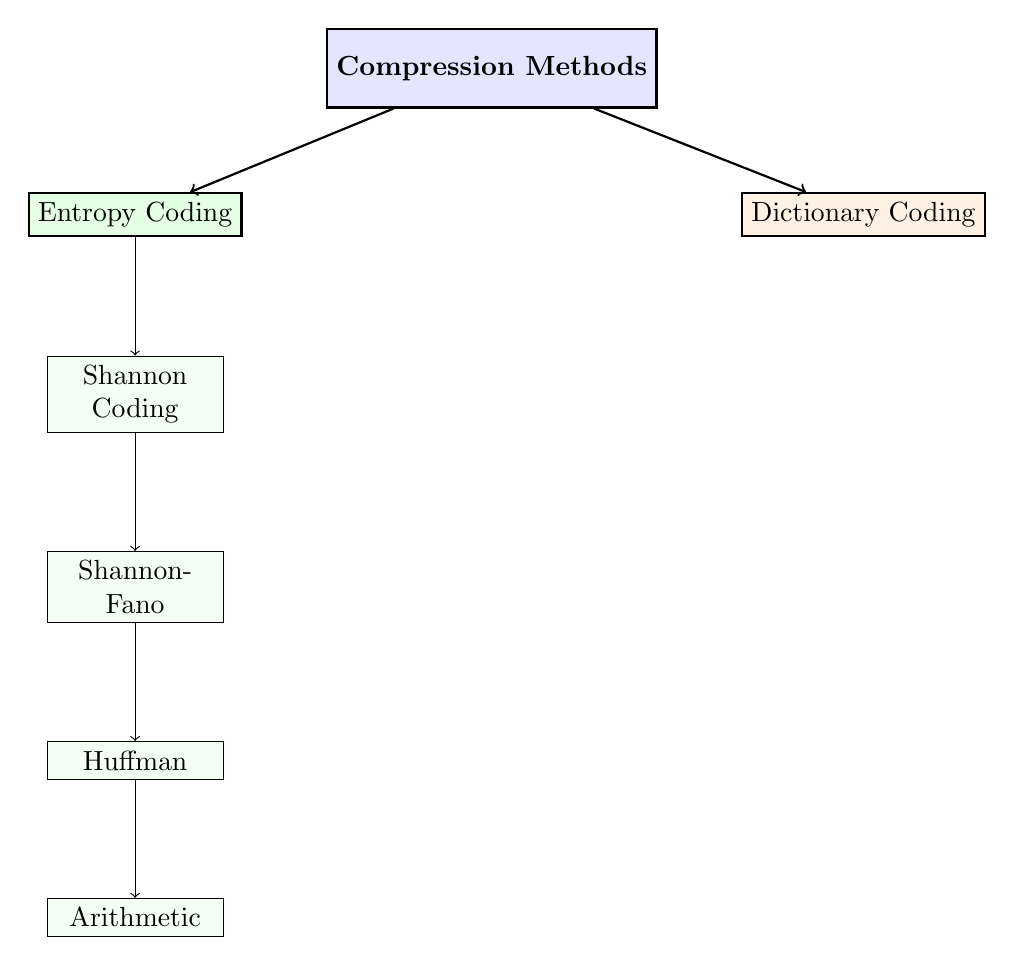
\begin{tikzpicture}[node distance=1.5cm]
\node (compression) [rectangle, draw=black, thick, fill=blue!10, minimum width=3cm, minimum height=1cm] {\textbf{Compression Methods}};
\node (entropy) [below left=of compression, rectangle, draw=black, thick, fill=green!10, minimum width=2.5cm] {Entropy Coding};
\node (dictionary) [below right=of compression, rectangle, draw=black, thick, fill=orange!10, minimum width=2.5cm] {Dictionary Coding};
\node (shannon) [below=of entropy, rectangle, draw=black, fill=green!5, text width=2cm, align=center] {Shannon Coding};
\node (shannonfano) [below=of shannon, rectangle, draw=black, fill=green!5, text width=2cm, align=center] {Shannon-Fano};
\node (huffman) [below=of shannonfano, rectangle, draw=black, fill=green!5, text width=2cm, align=center] {Huffman};
\node (arithmetic) [below=of huffman, rectangle, draw=black, fill=green!5, text width=2cm, align=center] {Arithmetic};

\draw[->, thick] (compression) -- (entropy);
\draw[->, thick] (compression) -- (dictionary);
\draw[->] (entropy) -- (shannon);
\draw[->] (shannon) -- (shannonfano);
\draw[->] (shannonfano) -- (huffman);
\draw[->] (huffman) -- (arithmetic);
\end{tikzpicture}
\end{center}

\textbf{Key Dimensions in Coding Taxonomy:}

\begin{enumerate}
    \item \textbf{Modeling vs. Coding Separation:}
    \begin{itemize}
        \item \textbf{Modeling}: Probability estimation of symbols
        \item \textbf{Coding}: Assigning bit sequences based on probabilities
    \end{itemize}
    
    \item \textbf{Static vs. Adaptive vs. Universal:}
    \begin{itemize}
        \item \textbf{Static}: Fixed probabilities known in advance
        \item \textbf{Adaptive}: Probabilities updated during encoding
        \item \textbf{Universal}: Adapts to unknown distributions
    \end{itemize}
    
    \item \textbf{Block Codes vs. Stream Codes:}
    \begin{itemize}
        \item \textbf{Block}: Fixed-length input blocks
        \item \textbf{Stream}: Continuous data processing
    \end{itemize}
    
    \item \textbf{Symbol-by-Symbol vs. Message-Wide:}
    \begin{itemize}
        \item \textbf{Symbol-by-symbol}: Each symbol coded independently (Huffman)
        \item \textbf{Message-wide}: Entire message coded as one unit (Arithmetic)
    \end{itemize}
\end{enumerate}

\subsection{Shannon Coding (1948)}

\begin{definitionbox}
\textbf{Shannon Coding:} A constructive method derived from Shannon's source coding theorem:
\[
l_i = \lceil -\log_2 p_i \rceil
\]
where $p_i$ is the probability of symbol $i$.
\end{definitionbox}

\begin{examplebox}
\textbf{Example:} Given symbols with probabilities:
\begin{center}
\begin{tabular}{c|c|c}
Symbol & Probability & $-\log_2 p_i$ \\
\hline
A & 0.5 & 1.0 \\
B & 0.25 & 2.0 \\
C & 0.125 & 3.0 \\
D & 0.125 & 3.0 \\
\end{tabular}
\end{center}

\textbf{Shannon code construction:}
\begin{enumerate}
    \item Calculate lengths: $l_A = \lceil 1.0 \rceil = 1$, $l_B = 2$, $l_C = 3$, $l_D = 3$
    \item Sort by probability (decreasing)
    \item Assign cumulative probabilities: $F_A=0$, $F_B=0.5$, $F_C=0.75$, $F_D=0.875$
    \item Convert $F_i$ to binary with $l_i$ bits:
    \begin{itemize}
        \item A: $0.0_2 \rightarrow 0$
        \item B: $0.5_{10} = 0.1_2 \rightarrow 10$
        \item C: $0.75_{10} = 0.11_2 \rightarrow 110$
        \item D: $0.875_{10} = 0.111_2 \rightarrow 111$
    \end{itemize}
\end{enumerate}
\textbf{Expected length:} $L = 0.5\times1 + 0.25\times2 + 0.125\times3 + 0.125\times3 = 1.75$ bits/symbol
\end{examplebox}

\begin{importantbox}
\textbf{Properties of Shannon Coding:}
\begin{itemize}
    \item \textbf{Constructive proof}: Demonstrates Kraft-McMillan inequality
    \item \textbf{Simple to compute}: Direct from probabilities
    \item \textbf{Not optimal}: Unlike Huffman, doesn't minimize expected length
    \item \textbf{Theoretical importance}: Foundation for Shannon's theorem
\end{itemize}
\end{importantbox}

\subsection{Shannon-Fano Coding (1949)}

\begin{definitionbox}
\textbf{Shannon-Fano Coding:} A top-down recursive splitting method developed independently by Shannon and Fano.
\end{definitionbox}

\begin{algorithm}
\caption{Shannon-Fano Coding Algorithm}
\begin{algorithmic}[1]
\REQUIRE Symbols with probabilities $p_1 \geq p_2 \geq \cdots \geq p_n$
\ENSURE Prefix code for each symbol
\STATE Sort symbols by decreasing probability
\STATE \textbf{function} SF($symbols$)
    \IF{$|symbols| = 1$}
        \RETURN (assign empty code)
    \ENDIF
    \STATE Split $symbols$ into two subsets $S_1$ and $S_2$ with nearly equal total probabilities
    \STATE Append '0' to codes of symbols in $S_1$
    \STATE Append '1' to codes of symbols in $S_2$
    \STATE SF($S_1$)
    \STATE SF($S_2$)
\STATE \textbf{end function} % FIXED: Changed \ENDFUNCTION to proper syntax
\end{algorithmic}
\end{algorithm}

\begin{examplebox}
\textbf{Example:} Same symbols as before:
\begin{center}
\begin{tabular}{c|c}
Symbol & Probability \\
\hline
A & 0.5 \\
B & 0.25 \\
C & 0.125 \\
D & 0.125 \\
\end{tabular}
\end{center}

\textbf{Construction:}
\begin{enumerate}
    \item Split 1: $\{A\}(0.5)$ vs $\{B,C,D\}(0.5)$ → A:0, others:1
    \item Split 2: $\{B\}(0.25)$ vs $\{C,D\}(0.25)$ → B:10, others:11
    \item Split 3: $\{C\}(0.125)$ vs $\{D\}(0.125)$ → C:110, D:111
\end{enumerate}

\textbf{Codes:} A=0, B=10, C=110, D=111 \\
\textbf{Expected length:} Same as Huffman in this case: 1.75 bits/symbol
\end{examplebox}

\begin{importantbox}
\textbf{Historical Note:} Shannon-Fano coding was developed before Huffman coding (1952). While simpler conceptually, it is \textbf{not always optimal}. Huffman's bottom-up approach guarantees optimality for given probabilities.
\end{importantbox}

\subsection{Canonical Huffman Codes}

\begin{definitionbox}
\textbf{Canonical Huffman Code:} A Huffman code where codes are assigned in a specific canonical (standard) form, enabling more efficient representation and faster decoding.
\end{definitionbox}

\begin{algorithm}
\caption{Canonical Huffman Construction}
\begin{algorithmic}[1]
\REQUIRE Symbol code lengths $l_i$ from standard Huffman
\ENSURE Canonical Huffman codes
\STATE Sort symbols by: (1) code length $l_i$, (2) symbol value
\STATE Assign first code: $code = 0$ (in binary with $l_{min}$ bits)
\FOR{each symbol in sorted order}
    \STATE Assign current $code$ to symbol
    \STATE Increment $code$ by 1
    \IF{next symbol has longer code length}
        \STATE Left-shift $code$ by difference in lengths
    \ENDIF
\ENDFOR
\end{algorithmic}
\end{algorithm}

\begin{examplebox}
\textbf{Example:} Suppose Huffman gives these lengths:
\begin{center}
\begin{tabular}{c|c|c}
Symbol & Length & Original Huffman \\
\hline
A & 2 & 00 \\
B & 3 & 010 \\
C & 3 & 011 \\
D & 3 & 100 \\
E & 4 & 1010 \\
F & 4 & 1011 \\
\end{tabular}
\end{center}

\textbf{Canonical construction:}
\begin{enumerate}
    \item Sort: A(2), B(3), C(3), D(3), E(4), F(4)
    \item Start: A gets code 00 (binary 0 in 2 bits)
    \item Increment: B gets 010 (binary 2 in 3 bits: 010)
    \item Increment: C gets 011 (binary 3: 011)
    \item Increment: D gets 100 (binary 4: 100)
    \item For E: length increases to 4, so left-shift: 100 → 1000
    \item Increment: F gets 1001
\end{enumerate}

\textbf{Canonical codes:} A=00, B=010, C=011, D=100, E=1000, F=1001
\end{examplebox}

\begin{importantbox}
\textbf{Advantages of Canonical Huffman:}
\begin{itemize}
    \item \textbf{Compact representation}: Only need to store code lengths, not the full tree
    \item \textbf{Fast decoding}: Use table-based lookup instead of tree traversal
    \item \textbf{Standardized}: Used in DEFLATE (ZIP, gzip), JPEG, PNG, MPEG
\end{itemize}

\textbf{Transmission:} Send only: $\langle$symbol count, lengths$\rangle$ instead of full tree
\end{importantbox}

\subsection{Adaptive Huffman Coding}

\begin{definitionbox}
\textbf{Adaptive Huffman Coding:} Dynamically updates the Huffman tree as symbols are processed, requiring only one pass over the data.
\end{definitionbox}

\textbf{Key Algorithms:}
\begin{itemize}
    \item \textbf{FGK Algorithm} (Faller, Gallager, Knuth, 1978)
    \item \textbf{Vitter's Algorithm} (1987) - more efficient
\end{itemize}

\begin{importantbox}
\textbf{How it works:}
\begin{enumerate}
    \item Start with empty tree or initial estimates
    \item For each symbol:
    \begin{itemize}
        \item Encode using current tree
        \item Update symbol frequency
        \item Reconstruct/update tree incrementally
    \end{itemize}
    \item Sibling property maintained for optimality
\end{enumerate}
\end{importantbox}

\textbf{Applications:} Early UNIX compress utility, network protocols where distribution changes.

\subsection{Arithmetic Coding: The Paradigm Shift}

\begin{definitionbox}
\textbf{Arithmetic Coding:} Encodes an entire message into a single fractional number in the interval $[0,1)$, approaching the entropy bound very closely.
\end{definitionbox}

\textbf{Core Idea:} Represent messages as subintervals of $[0,1)$:

\begin{center}
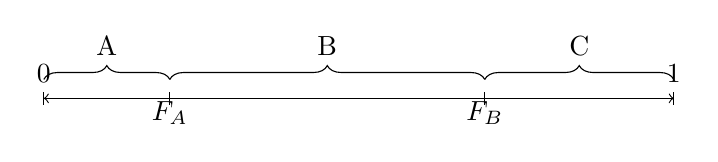
\begin{tikzpicture}[scale=0.8]
\draw[<->] (0,0) -- (10,0);
\draw (0,-0.1) -- (0,0.1) node[above] {0};
\draw (10,-0.1) -- (10,0.1) node[above] {1};
\draw (2,-0.1) -- (2,0.1) node[below] {$F_{A}$};
\draw (7,-0.1) -- (7,0.1) node[below] {$F_{B}$};
\draw[decorate,decoration={brace,amplitude=5pt}] (0,0.3) -- (2,0.3) node[midway,above=5pt] {A};
\draw[decorate,decoration={brace,amplitude=5pt}] (2,0.3) -- (7,0.3) node[midway,above=5pt] {B};
\draw[decorate,decoration={brace,amplitude=5pt}] (7,0.3) -- (10,0.3) node[midway,above=5pt] {C};
\end{tikzpicture}
\end{center}

\begin{algorithm}
\caption{Arithmetic Encoding Algorithm}
\begin{algorithmic}[1]
\REQUIRE Message $m = s_1 s_2 \dots s_k$, symbol probabilities $p_i$
\ENSURE Final interval $[low, high)$
\STATE $low \gets 0.0$, $high \gets 1.0$
\FOR{each symbol $s$ in $m$}
    \STATE $range \gets high - low$
    \STATE $high \gets low + range \times F_s$ \COMMENT{$F_s$: cumulative prob up to $s$}
    \STATE $low \gets low + range \times F_{s-1}$ \COMMENT{$F_{s-1}$: cumulative prob before $s$}
\ENDFOR
\RETURN any number in $[low, high)$
\end{algorithmic}
\end{algorithm}

\begin{examplebox}
\textbf{Example:} Encode message "CAB" with probabilities: A(0.5), B(0.25), C(0.25)

\begin{center}
\begin{tabular}{c|c|c}
Symbol & Probability & Cumulative \\
\hline
A & 0.5 & 0.5 \\
B & 0.25 & 0.75 \\
C & 0.25 & 1.0 \\
\end{tabular}
\end{center}

\textbf{Encoding:}
\begin{enumerate}
    \item Start: $[0, 1)$
    \item Process 'C': $[0.75, 1.0)$ \quad (C occupies $[0.75, 1.0)$)
    \item Process 'A': $range = 0.25$
        \begin{itemize}
            \item $low = 0.75 + 0.25 \times 0.0 = 0.75$
            \item $high = 0.75 + 0.25 \times 0.5 = 0.875$
            \item New interval: $[0.75, 0.875)$
        \end{itemize}
    \item Process 'B': $range = 0.125$
        \begin{itemize}
            \item $low = 0.75 + 0.125 \times 0.5 = 0.8125$
            \item $high = 0.75 + 0.125 \times 0.75 = 0.84375$
            \item Final interval: $[0.8125, 0.84375)$
        \end{itemize}
\end{enumerate}
\textbf{Output:} Any number in $[0.8125, 0.84375)$, e.g., 0.8125 in binary
\end{examplebox}

\begin{importantbox}
\textbf{Practical Implementation Issues:}
\begin{itemize}
    \item \textbf{Finite precision}: Use integer arithmetic with scaling
    \item \textbf{Renormalization}: Output bits when interval confined to one half
    \item \textbf{Carry-over}: Handle when interval spans midpoint
    \item \textbf{Termination}: Need special end-of-message symbol
\end{itemize}
\end{importantbox}

\textbf{Adaptive Arithmetic Coding:} Easier than adaptive Huffman - just update probabilities as you go!

\subsection{Comparison \& Synthesis}

% Fixed table to fit within margins
\begin{center}
\small % Use smaller font for table
\begin{tabular}{|p{2.5cm}|c|c|c|c|p{2.5cm}|}
\hline
\textbf{Method} & \textbf{Optimal?} & \textbf{Adaptive?} & \textbf{Complexity} & \textbf{Near Entropy?} & \textbf{Key Applications} \\
\hline
Shannon Coding & No & No & Low & No & Theoretical proofs \\
\hline
Shannon-Fano & No & No & Low & Sometimes & Historical \\
\hline
Huffman & Yes* & No & Low & Moderate & General purpose \\
\hline
Canonical Huffman & Yes* & No & Low & Moderate & DEFLATE, JPEG, PNG \\
\hline
Adaptive Huffman & Yes* & Yes & Medium & Moderate & Early compressors \\
\hline
Arithmetic Coding & \textbf{Near-opt} & \textbf{Yes} & \textbf{High} & \textbf{Yes (close)} & \textbf{JPEG2000, H.264, HEVC} \\
\hline
\end{tabular}
\end{center}
\smallskip
*Optimal for symbol-by-symbol coding given probabilities

\begin{importantbox}
\textbf{Key Insights:}
\begin{itemize}
    \item \textbf{Huffman vs. Arithmetic}: Huffman is simpler but has an "integer penalty"; Arithmetic approaches entropy bound
    \item \textbf{Modern standards}: Arithmetic coding (CABAC) used in video compression for 10-20\% better compression
    \item \textbf{Practical choice}: For general compression, Canonical Huffman (DEFLATE); for media, Arithmetic coding
    \item \textbf{The missing piece}: All these methods assume we have good probability estimates. Where do those come from?
\end{itemize}
\end{importantbox}

\subsection{Forward Look}

\textbf{The Complete Picture: What Comes Next?}

\begin{center}
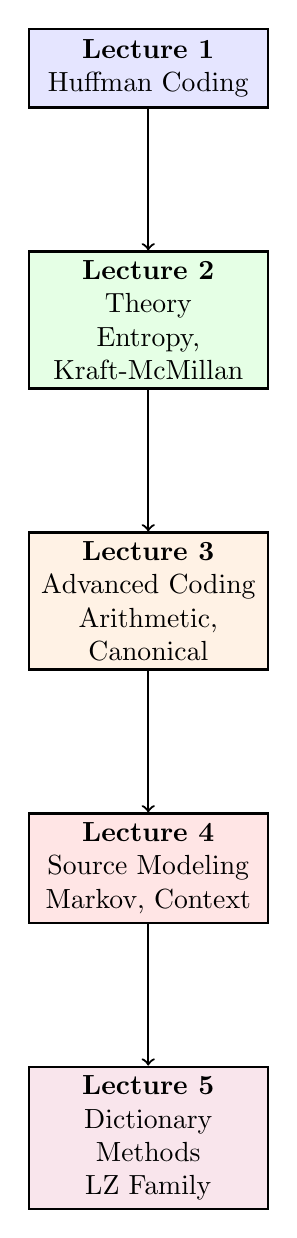
\begin{tikzpicture}[node distance=1.8cm]
\node (lecture1) [rectangle, draw=black, thick, fill=blue!10, minimum width=3cm, minimum height=1cm] {\parbox{2.8cm}{\centering \textbf{Lecture 1}\\Huffman Coding}};
\node (lecture2) [below=of lecture1, rectangle, draw=black, thick, fill=green!10, minimum width=3cm, minimum height=1cm] {\parbox{2.8cm}{\centering \textbf{Lecture 2}\\Theory\\Entropy, Kraft-McMillan}};
\node (lecture3) [below=of lecture2, rectangle, draw=black, thick, fill=orange!10, minimum width=3cm, minimum height=1cm] {\parbox{2.8cm}{\centering \textbf{Lecture 3}\\Advanced Coding\\Arithmetic, Canonical}};
\node (lecture4) [below=of lecture3, rectangle, draw=black, thick, fill=red!10, minimum width=3cm, minimum height=1cm] {\parbox{2.8cm}{\centering \textbf{Lecture 4}\\Source Modeling\\Markov, Context}};
\node (lecture5) [below=of lecture4, rectangle, draw=black, thick, fill=purple!10, minimum width=3cm, minimum height=1cm] {\parbox{2.8cm}{\centering \textbf{Lecture 5}\\Dictionary Methods\\LZ Family}};

\draw[->, thick] (lecture1) -- (lecture2);
\draw[->, thick] (lecture2) -- (lecture3);
\draw[->, thick] (lecture3) -- (lecture4);
\draw[->, thick] (lecture4) -- (lecture5);
\end{tikzpicture}
\end{center}

\textbf{Next Lecture: Source Modeling and Statistical Dependence}
\begin{itemize}
    \item \textbf{The missing half}: We now know how to code efficiently, but where do the probabilities come from?
    \item \textbf{Real data has memory}: 'Q' is usually followed by 'U' in English text
    \item \textbf{Markov models}: Capturing dependencies between symbols
    \item \textbf{Context modeling}: Using past symbols to predict future ones
    \item \textbf{The modeling-coding separation}: Modern compressors separate these two tasks
\end{itemize}

\textbf{The Big Question for Next Time:}
\begin{center}
\fbox{\parbox{0.8\textwidth}{\centering
\textbf{If Arithmetic coding can get within 0.01 bits of entropy,\\ 
what's the real limit to compression?\\ 
The answer: It's not the coding, it's the \textit{modeling}!}}
}
\end{center}

\textbf{The Two Pillars of Compression (Revised View):}
\begin{center}
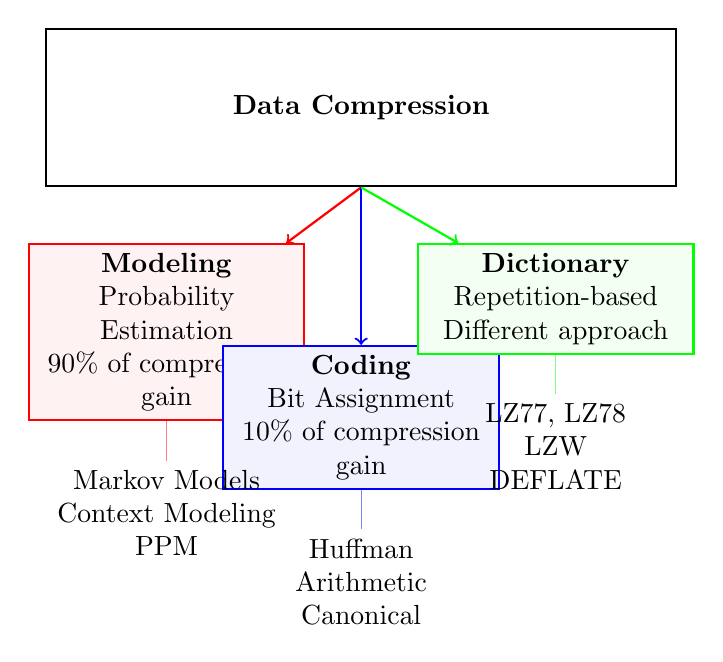
\begin{tikzpicture}[node distance=2cm]
\node (comp) [rectangle, draw=black, thick, minimum width=8cm, minimum height=2cm] {\textbf{Data Compression}};
\node (modeling) [below left=1cm of comp.south, rectangle, draw=red, thick, fill=red!5, minimum width=3.5cm, minimum height=1.2cm] {\parbox{3.2cm}{\centering \textbf{Modeling}\\Probability Estimation\\90\% of compression gain}};
\node (coding) [below=of comp, rectangle, draw=blue, thick, fill=blue!5, minimum width=3.5cm, minimum height=1.2cm] {\parbox{3.2cm}{\centering \textbf{Coding}\\Bit Assignment\\10\% of compression gain}};
\node (dictionary) [below right=1cm of comp.south, rectangle, draw=green, thick, fill=green!5, minimum width=3.5cm, minimum height=1.2cm] {\parbox{3.2cm}{\centering \textbf{Dictionary}\\Repetition-based\\Different approach}};

\draw[->, thick, red] (comp.south) -- (modeling);
\draw[->, thick, blue] (comp.south) -- (coding);
\draw[->, thick, green] (comp.south) -- (dictionary);

\node (modeltech) [below=0.5cm of modeling] {\parbox{3.2cm}{\centering Markov Models\\Context Modeling\\PPM}};
\node (codetech) [below=0.5cm of coding] {\parbox{3.2cm}{\centering Huffman\\Arithmetic\\Canonical}};
\node (dicttech) [below=0.5cm of dictionary] {\parbox{3.2cm}{\centering LZ77, LZ78\\LZW\\DEFLATE}};

\draw[red!50] (modeling) -- (modeltech);
\draw[blue!50] (coding) -- (codetech);
\draw[green!50] (dictionary) -- (dicttech);
\end{tikzpicture}
\end{center}

\begin{exercisebox}
\textbf{Exercise 3.1:} Given symbols with probabilities: A(0.4), B(0.3), C(0.2), D(0.1)
\begin{enumerate}[label=(\alph*)]
    \item Construct a Shannon code and compute its expected length
    \item Construct a Shannon-Fano code
    \item Compare with Huffman code from Lecture 2
\end{enumerate}
\end{exercisebox}

\begin{exercisebox}
\textbf{Exercise 3.2:} Convert the following Huffman code to canonical form:
\begin{center}
\begin{tabular}{c|c}
Symbol & Huffman Code \\
\hline
A & 0 \\
B & 100 \\
C & 101 \\
D & 110 \\
E & 1110 \\
F & 1111 \\
\end{tabular}
\end{center}
\end{exercisebox}

\begin{exercisebox}
\textbf{Exercise 3.3:} Encode the message "ABAC" using arithmetic coding with probabilities: A(0.6), B(0.3), C(0.1). Show each step.
\end{exercisebox}

\begin{exercisebox}
\textbf{Exercise 3.4: Thinking Ahead:} Consider the English phrase "THE QUICK BROWN FOX"
\begin{enumerate}[label=(\alph*)]
    \item If we use Huffman coding with letter frequencies, what's wrong with this approach?
    \item How might knowing that 'Q' is usually followed by 'U' help compression?
    \item Why would arithmetic coding be better than Huffman for this kind of data?
\end{enumerate}
\end{exercisebox}

\vspace{1cm}
\begin{center}
\rule{0.8\textwidth}{0.5pt}\\
\textbf{End of Lecture 3 -- Advanced Entropy Coding Methods}\\
\textbf{Next: Lecture 4 -- Source Modeling and Statistical Dependence}\\
\textit{We now have efficient coding methods. Next: Where do the probabilities come from?}
\end{center}

\newpage
% File: lecture_4.tex
\section{Source Modeling and Statistical Dependence}

\begin{center}
\textbf{Lecture 4: Beyond Coding -- The Power of Source Modeling}
\end{center}

\subsection{Introduction: Beyond Coding}

\begin{importantbox}
\textbf{Key Insight:} In the first three lectures, we've focused on \textbf{coding} - efficient ways to represent symbols given their probabilities. Now we address the other half: \textbf{modeling} - how to get good probability estimates in the first place.
\end{importantbox}

\textbf{The Big Picture:}

\begin{center}
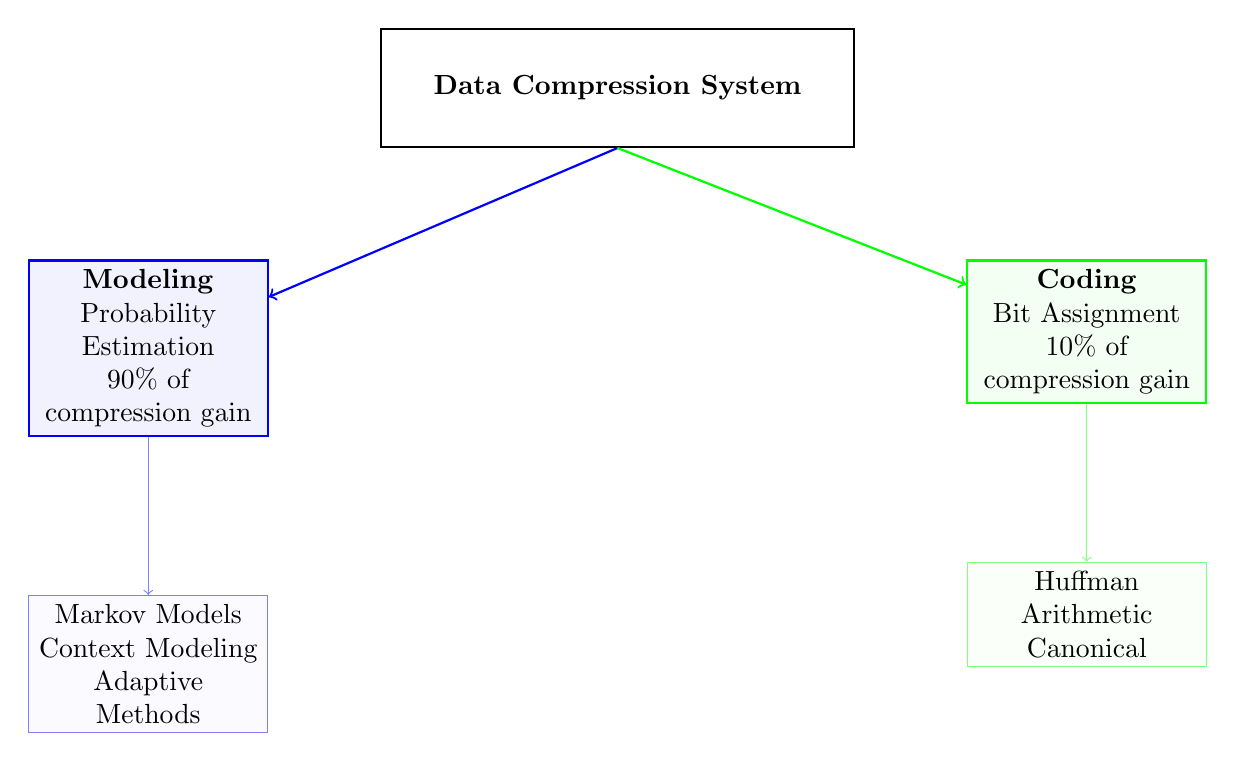
\begin{tikzpicture}[node distance=2cm]
\node (compress) [rectangle, draw=black, thick, minimum width=6cm, minimum height=1.5cm] {\textbf{Data Compression System}};
\node (model) [below left=of compress, rectangle, draw=blue, thick, fill=blue!5, minimum width=3cm, minimum height=1cm] {\parbox{2.8cm}{\centering \textbf{Modeling}\\Probability Estimation\\90\% of compression gain}};
\node (code) [below right=of compress, rectangle, draw=green, thick, fill=green!5, minimum width=3cm, minimum height=1cm] {\parbox{2.8cm}{\centering \textbf{Coding}\\Bit Assignment\\10\% of compression gain}};
\node (modeltech) [below=of model, rectangle, draw=blue!50, fill=blue!2, text width=2.8cm, align=center] {Markov Models\\Context Modeling\\Adaptive Methods};
\node (codetech) [below=of code, rectangle, draw=green!50, fill=green!2, text width=2.8cm, align=center] {Huffman\\Arithmetic\\Canonical};

\draw[->, thick, blue] (compress.south) -- (model);
\draw[->, thick, green] (compress.south) -- (code);
\draw[->, blue!50] (model) -- (modeltech);
\draw[->, green!50] (code) -- (codetech);
\end{tikzpicture}
\end{center}

\textbf{Why Real Data Defies IID Assumptions:}
\begin{itemize}
    \item \textbf{IID (Independent Identically Distributed)}: Assumption behind simple Huffman
    \item \textbf{Reality}: Data has \textbf{memory} and \textbf{dependencies}
    \item Example: In English text, 'Q' is almost always followed by 'U'
    \item Example: In images, neighboring pixels are highly correlated
\end{itemize}

\textbf{Today's Roadmap:}
\begin{enumerate}
    \item Understand statistical dependence in data
    \item Learn Markov models for capturing memory
    \item Explore context modeling techniques
    \item See practical examples with real data
    \item Connect modeling to coding (Lecture 3)
\end{enumerate}

\subsection{Memoryless vs. Sources with Memory}

\begin{definitionbox}
\textbf{Memoryless Source (IID):} Each symbol is generated independently of all previous symbols. Probability distribution: $P(X_n = x) = p(x)$ for all $n$.
\end{definitionbox}

\begin{definitionbox}
\textbf{Source with Memory:} The probability of a symbol depends on previous symbols. Example: $P(X_n = x | X_{n-1} = y, X_{n-2} = z, \dots)$.
\end{definitionbox}

\begin{examplebox}
\textbf{Examples of Dependence in Real Data:}
\begin{itemize}
    \item \textbf{Text}: 'TH' is common, 'TQ' is rare
    \item \textbf{Images}: Neighboring pixels have similar colors
    \item \textbf{Audio}: Sound waves have temporal continuity
    \item \textbf{Video}: Consecutive frames are nearly identical
    \item \textbf{Source code}: Keywords, variable names repeat
\end{itemize}
\end{examplebox}

\begin{importantbox}
\textbf{Measuring Dependence: Autocorrelation}
\[
\rho(k) = \frac{\mathbb{E}[(X_t - \mu)(X_{t+k} - \mu)]}{\sigma^2}
\]
where $k$ is the lag. High $\rho(k)$ means strong dependence at distance $k$.
\end{importantbox}

\subsection{Conditional Entropy and Mutual Information}

\begin{definitionbox}
\textbf{Conditional Entropy:} The average uncertainty about $X$ given knowledge of $Y$:
\[
H(X|Y) = -\sum_{x \in \mathcal{X}} \sum_{y \in \mathcal{Y}} p(x,y) \log_2 p(x|y)
\]
\end{definitionbox}

\begin{examplebox}
\textbf{Intuition: "Knowing the Past Helps Predict the Future"}\\
Consider English letters:
\begin{itemize}
    \item Unconditional: $H(\text{letter}) \approx 4.07$ bits
    \item Given previous letter: $H(\text{letter}|\text{previous}) \approx 3.36$ bits
    \item Given previous 2 letters: $H(\text{letter}|\text{previous 2}) \approx 2.77$ bits
\end{itemize}
Each additional letter of context reduces uncertainty!
\end{examplebox}

\begin{definitionbox}
\textbf{Mutual Information:} Measures how much knowing $Y$ reduces uncertainty about $X$:
\[
I(X;Y) = H(X) - H(X|Y) = H(Y) - H(Y|X)
\]
\end{definitionbox}

\begin{examplebox}
\textbf{Worked Example: English Letter Dependence}\\
Let $X$ = current letter, $Y$ = previous letter.
\begin{align*}
H(X) &= 4.07 \text{ bits} \\
H(X|Y) &= 3.36 \text{ bits} \\
I(X;Y) &= 4.07 - 3.36 = 0.71 \text{ bits}
\end{align*}
This means knowing the previous letter gives us 0.71 bits of information about the current letter.
\end{examplebox}

\subsection{Markov Sources}

\begin{definitionbox}
\textbf{Markov Property (Memory-$m$):} The future depends only on the last $m$ symbols:
\[
P(X_n = x | X_{n-1}, X_{n-2}, \dots, X_1) = P(X_n = x | X_{n-1}, \dots, X_{n-m})
\]
\end{definitionbox}

\textbf{First-Order Markov Model ($m=1$):}
\begin{itemize}
    \item Only the immediately previous symbol matters
    \item Represented by transition probabilities $p_{ij} = P(X_n = j | X_{n-1} = i)$
    \item Can be shown as a state diagram or transition matrix
\end{itemize}

\begin{examplebox}
\textbf{Example: Weather Prediction Markov Chain}\\
States: $\{\text{Sunny (S)}, \text{Rainy (R)}\}$\\
Transition probabilities:
\begin{center}
\begin{tabular}{c|cc}
 & S & R \\
\hline
S & 0.8 & 0.2 \\
R & 0.3 & 0.7 \\
\end{tabular}
\end{center}
Interpretation: If today is sunny, 80\% chance tomorrow is sunny, 20\% chance rainy.
\end{examplebox}

\textbf{Higher-Order Markov Models:}
\begin{itemize}
    \item Order-$k$: Depends on last $k$ symbols
    \item More accurate but exponentially more parameters
    \item Number of parameters grows as $|\mathcal{A}|^{k+1}$ where $\mathcal{A}$ is alphabet size
\end{itemize}

\begin{importantbox}
\textbf{Memory-Complexity Trade-off:}
\begin{itemize}
    \item \textbf{Order 0}: 26 parameters for English (simple but weak)
    \item \textbf{Order 1}: $26 \times 26 = 676$ parameters
    \item \textbf{Order 2}: $26 \times 26 \times 26 = 17,576$ parameters
    \item \textbf{Order 5}: $26^6 \approx 308$ million parameters!
\end{itemize}
This is the \textbf{context explosion problem}.
\end{importantbox}

\subsection{Entropy Rate Revisited}

\begin{definitionbox}
\textbf{Entropy Rate of a Stationary Source:}

For a stationary stochastic process $\mathcal{X} = (X_1, X_2, \dots)$, the entropy rate is:
\[
H(\mathcal{X}) = \lim_{n \to \infty} \frac{1}{n} H(X_1, X_2, \dots, X_n)
\]
Equivalently (and equal for stationary processes):
\[
H(\mathcal{X}) = \lim_{n \to \infty} H(X_n \mid X_1, \dots, X_{n-1})
\]

\medskip
\textbf{Special case: Stationary Markov chain of order $m$}

If $\mathcal{X}$ is a stationary $m$-th order Markov chain, then for all $t > m$:
\[
H(X_t \mid X_1, \dots, X_{t-1}) = H(X_t \mid X_{t-m}, \dots, X_{t-1})
\]
and this conditional entropy is constant over time. Therefore:
\[
H(\mathcal{X}) = H(X_{m+1} \mid X_1, \dots, X_m)
\]
No limit needed — the conditional entropy stabilizes immediately.
\end{definitionbox}

\begin{examplebox}
\textbf{Example: First-Order Markov Chain ($m=1$)}

\textbf{Step 1: Define the model}
Two weather states: $S$ (sunny) and $R$ (rainy). \\
\textbf{Transition probabilities} (tomorrow's weather depends only on today's):

Let $X_t$ be the weather on day $t$. Then:

\[
\begin{aligned}
P(X_{t+1} = S \mid X_t = S) &= 0.8, &\quad P(X_{t+1} = R \mid X_t = S) &= 0.2 \\
P(X_{t+1} = S \mid X_t = R) &= 0.3, &\quad P(X_{t+1} = R \mid X_t = R) &= 0.7
\end{aligned}
\]

In matrix form (rows = current state, columns = next state):
\[
P = \begin{bmatrix}
0.8 & 0.2 \\
0.3 & 0.7
\end{bmatrix}
\quad
\begin{array}{l}
\text{Row 1: } X_t = S \\
\text{Row 2: } X_t = R
\end{array}
\]

\textbf{Step 2: Find stationary distribution $\pi$}
Stationary distribution $\pi = [\pi_S, \pi_R]$ satisfies $\pi P = \pi$, where $\pi_S = P(X_t = S)$ and $\pi_R = P(X_t = R)$ in the long run.

\[
\begin{cases}
\pi_S = 0.8\pi_S + 0.3\pi_R \\
\pi_R = 0.2\pi_S + 0.7\pi_R \\
\pi_S + \pi_R = 1
\end{cases}
\]

Solving (from first equation): 
\[
\pi_S - 0.8\pi_S = 0.3\pi_R \Rightarrow 0.2\pi_S = 0.3\pi_R \Rightarrow \pi_S = 1.5\pi_R
\]
\[
1.5\pi_R + \pi_R = 1 \Rightarrow 2.5\pi_R = 1 \Rightarrow \pi_R = 0.4
\]
\[
\pi_S = 1.5 \times 0.4 = 0.6
\]

\[
\pi = [\pi_S, \pi_R] = [0.6, 0.4]
\]

\textbf{Step 3: Compute conditional entropies}
\textit{Uncertainty about tomorrow given today's weather:}

Given $X_t = S$: Tomorrow's distribution is $[0.8, 0.2]$
\[
H(X_{t+1} \mid X_t = S) = -0.8\log_2 0.8 - 0.2\log_2 0.2 \approx 0.7219 \text{ bits}
\]

Given $X_t = R$: Tomorrow's distribution is $[0.3, 0.7]$
\[
H(X_{t+1} \mid X_t = R) = -0.3\log_2 0.3 - 0.7\log_2 0.7 \approx 0.8813 \text{ bits}
\]

\textbf{Step 4: Compute entropy rate}
For a stationary first-order Markov chain:
\[
H(\mathcal{X}) = H(X_{t+1} \mid X_t) 
= \sum_{s \in \{S,R\}} P(X_t = s) \cdot H(X_{t+1} \mid X_t = s)
\]

With $P(X_t = s) = \pi_s$ (stationarity):
\[
H(\mathcal{X}) = \pi_S \cdot H(X_{t+1} \mid X_t = S) + \pi_R \cdot H(X_{t+1} \mid X_t = R)
\]
\[
= 0.6 \times 0.7219 + 0.4 \times 0.8813 = 0.43314 + 0.35252 = 0.78566 \text{ bits}
\]
\[
\approx 0.786 \text{ bits per day}
\]

\end{examplebox}

\begin{importantbox}
\textbf{What This Means for Data Compression:}

\textbf{Two approaches to compression:}

\begin{enumerate}
    \item \textbf{IID (Independent Identically Distributed) assumption:}
    \begin{itemize}
        \item Treat each symbol as independent of previous ones
        \item Best achievable rate: $H(X)$ (marginal entropy)
        \item Example: English letters $\approx 4.07$ bits/letter
    \end{itemize}
    
    \item \textbf{With modeling (using context):}
    \begin{itemize}
        \item Account for dependencies between symbols (Markov structure)
        \item Use conditional probabilities based on previous symbols
        \item Best achievable rate: $H(\mathcal{X})$ (entropy rate)
        \item Example: English text $\approx 2.3$ bits/letter
    \end{itemize}
\end{enumerate}

\medskip
\textbf{Compression gain:}
\[
\frac{H(X) - H(\mathcal{X})}{H(X)} \approx \frac{4.07 - 2.3}{4.07} \approx 43\%
\]
Up to $\sim 45\%$ better compression by exploiting dependencies!

\end{importantbox}

\subsection{Context Modeling in Practice}

\begin{definitionbox}
\textbf{Context Modeling:} Maintain separate probability distributions for each possible context (history).
\end{definitionbox}

\textbf{Fixed-Length vs. Variable-Length Contexts:}
\begin{itemize}
    \item \textbf{Fixed-length}: Always use last $k$ symbols as context
    \item \textbf{Variable-length}: Use longest matching context in database
    \item Example: PPM (Prediction by Partial Matching) uses variable-length
\end{itemize}

\begin{examplebox}
\textbf{The Context Explosion Problem:}\\
For English text (26 letters + space):
\begin{center}
\begin{tabular}{l|l|l}
Order & Contexts & Parameters \\
\hline
0 & 1 & 27 \\
1 & 27 & 729 \\
2 & 729 & 19,683 \\
3 & 19,683 & 531,441 \\
4 & 531,441 & 14,348,907 \\
5 & 14,348,907 & 387,420,489 \\
\end{tabular}
\end{center}
By order 5: 387 million parameters need estimation!
\end{examplebox}

\textbf{Solutions to Context Explosion:}
\begin{enumerate}
    \item \textbf{Escaping}: Fall back to lower-order model when context unseen
    \item \textbf{Blending}: Combine predictions from different order models
    \item \textbf{Pruning}: Remove low-frequency contexts
    \item \textbf{Adaptive methods}: Update probabilities as data arrives
\end{enumerate}

\subsection{Case Study: Text Compression Modeling}

\begin{examplebox}
\textbf{1. Entropy Estimates for English Text (Theoretical Limits)}

\begin{center}
\begin{tabular}{l|l|l}
\textbf{Model/Estimation Method} & \textbf{Bits/Letter} & \textbf{Year/Source} \\
\hline
Letter frequencies only (Order-0) & 4.07 & Shannon 1948 \\
+ 1st order Markov (bigrams) & 3.36 &  \\
+ 2nd order (trigrams) & 2.77 &  \\
+ 3rd order & 2.43 &  \\
Human prediction experiment & 1.3 & Shannon 1951 \\
Modern best estimates & 1.0–1.5 & Various studies \\
\end{tabular}
\end{center}

\textbf{2. Practical Compression Performance}

\begin{center}
\begin{tabular}{l|l|l}
\textbf{Compressor/Method} & \textbf{Bits/Letter} & \textbf{Notes} \\
\hline
gzip (LZ77 + Huffman) & 2.5–3.0 & Fast, widely used \\
bzip2 (BWT + MTF + Huffman) & 2.3–2.8 & Better but slower \\
PPMd & 2.1–2.4 & Context modeling \\
PAQ variants & 1.5–1.8 & State of the art, very slow \\
\end{tabular}
\end{center}

\textbf{Key insight:} Better models (using more context) → lower entropy → better compression. \\
But practical compressors face tradeoffs: memory, speed, and model complexity.
\end{examplebox}

\textbf{PPM (Prediction by Partial Matching):}
\begin{itemize}
    \item Uses \textbf{variable-length} contexts
    \item Tries highest-order model first
    \item Escapes to lower order if context unseen
    \item Blends probabilities from different orders
    \item State-of-the-art for text compression in 1990s
\end{itemize}

\begin{importantbox}
\textbf{Practical Entropy Reduction:}
\begin{align*}
\text{IID model (Huffman)} &: 4.07 \text{ bits/letter} \\
\text{With context modeling} &: 2.23 \text{ bits/letter} \\
\text{Improvement} &: 45\% \text{ better compression!}
\end{align*}
\end{importantbox}

\subsection{The Modeling–Coding Separation Principle}

\begin{definitionbox}
\textbf{Modeling–Coding Separation:} Modern compressors separate probability estimation (modeling) from bit assignment (coding).
\end{definitionbox}

\textbf{Historical Evolution:}
\begin{itemize}
    \item \textbf{Early}: Integrated (Huffman builds tree from frequencies)
    \item \textbf{Modern}: Separated (Model → Probabilities → Arithmetic Coder)
\end{itemize}

\begin{center}
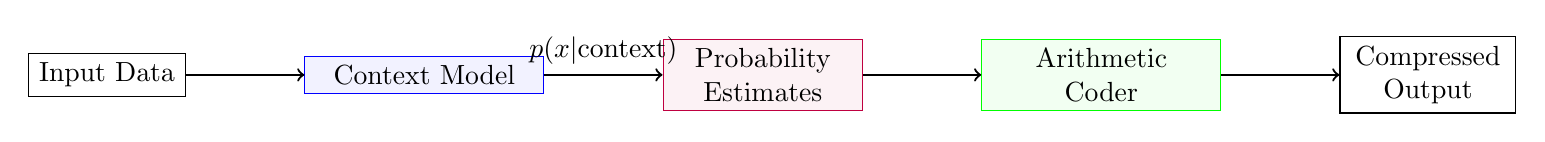
\begin{tikzpicture}[node distance=1.5cm]
\node (data) [rectangle, draw=black, minimum width=2cm] {Input Data};
\node (model) [right=of data, rectangle, draw=blue, fill=blue!5, minimum width=3cm] {\parbox{2.8cm}{\centering Context Model}};
\node (probs) [right=of model, rectangle, draw=purple, fill=purple!5, minimum width=2.5cm] {\parbox{2.3cm}{\centering Probability\\Estimates}};
\node (coder) [right=of probs, rectangle, draw=green, fill=green!5, minimum width=3cm] {\parbox{2.8cm}{\centering Arithmetic\\Coder}};
\node (output) [right=of coder, rectangle, draw=black, minimum width=2cm] {\parbox{2cm}{\centering Compressed\\Output}};

\draw[->, thick] (data) -- (model);
\draw[->, thick] (model) -- node[above] {$p(x|\text{context})$} (probs);
\draw[->, thick] (probs) -- (coder);
\draw[->, thick] (coder) -- (output);
\end{tikzpicture}
\end{center}

\begin{examplebox}
\textbf{How PPM + Arithmetic Beats Huffman:}
\begin{enumerate}
    \item \textbf{PPM}: Sees context "TH" → predicts E with 80\% probability
    \item \textbf{Arithmetic}: Encodes E using $p=0.8$ → ~0.32 bits
    \item \textbf{Huffman}: Would need at least 1 bit for any symbol
    \item \textbf{Gain}: 0.32 bits vs 1+ bits = 3× better for this symbol!
\end{enumerate}
\end{examplebox}

\begin{importantbox}
\textbf{Why Arithmetic Coding is the Perfect Backend:}
\begin{itemize}
    \item Can handle \textbf{fractional bits} per symbol
    \item Accepts \textbf{changing probabilities} symbol by symbol
    \item Works with \textbf{adaptive models} naturally
    \item Achieves entropy bound for good models
\end{itemize}
\end{importantbox}

\subsection{Adaptive vs. Static Modeling}

\begin{definitionbox}
\textbf{Static Models:} Train once on representative data, use fixed model for all files.
\begin{itemize}
    \item \textbf{Pros}: Fast encoding/decoding
    \item \textbf{Cons}: Model may not match specific file
    \item \textbf{Example}: Early text compressors using English statistics
\end{itemize}
\end{definitionbox}

\begin{definitionbox}
\textbf{Semi-Adaptive (Two-Pass):} First pass: collect statistics; Second pass: encode.
\begin{itemize}
    \item \textbf{Pros}: Tailored to specific file
    \item \textbf{Cons}: Need to transmit model (overhead)
    \item \textbf{Example}: Standard Huffman with tree transmission
\end{itemize}
\end{definitionbox}

\begin{definitionbox}
\textbf{Fully Adaptive (One-Pass):} Update model while encoding/decoding.
\begin{itemize}
    \item \textbf{Pros}: No model transmission, adapts to local changes
    \item \textbf{Cons}: Slower, initial poor compression
    \item \textbf{Example}: Adaptive Huffman, PPM with update
\end{itemize}
\end{definitionbox}

\begin{examplebox}
\textbf{Comparison in Practice:}
\begin{center}
\begin{tabular}{l|l|l|l}
Type & Compression & Speed & Memory \\
\hline
Static & Medium & Fast & Low \\
Semi-Adaptive & Good & Medium & Medium \\
Fully Adaptive & Best & Slow & High \\
\end{tabular}
\end{center}
Choice depends on application constraints!
\end{examplebox}

\subsection{Summary and Forward Look}

\begin{importantbox}
\textbf{Key Takeaways:}
\begin{enumerate}
    \item \textbf{The real compression is in modeling}, not just coding
    \item \textbf{Context matters}: Using past symbols reduces uncertainty
    \item \textbf{Markov models} capture memory in data
    \item \textbf{Context explosion} limits practical model order
    \item \textbf{Arithmetic coding} enables efficient use of good models
    \item \textbf{Adaptive methods} avoid model transmission overhead
\end{enumerate}
\end{importantbox}

\textbf{The Two Pillars Revisited:}

\begin{center}
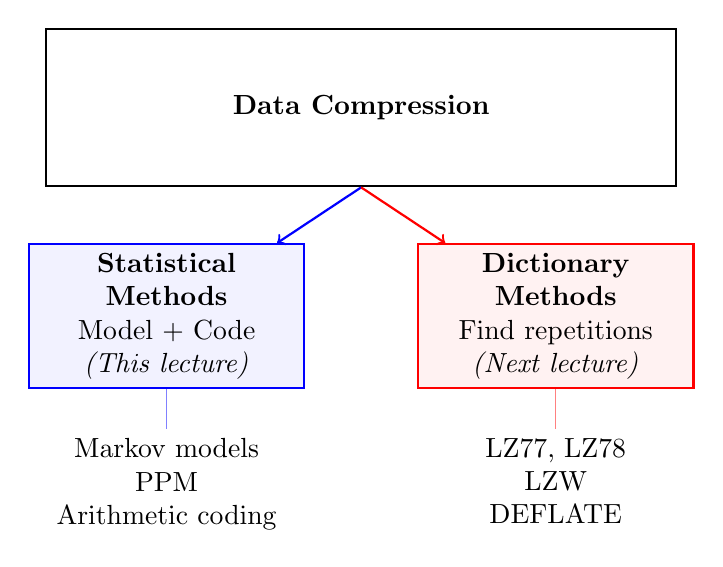
\begin{tikzpicture}[node distance=2cm]
\node (compress) [rectangle, draw=black, thick, minimum width=8cm, minimum height=2cm] {\textbf{Data Compression}};
\node (statistical) [below left=1cm of compress.south, rectangle, draw=blue, thick, fill=blue!5, minimum width=3.5cm, minimum height=1.2cm] {\parbox{3.2cm}{\centering \textbf{Statistical Methods}\\Model + Code\\\textit{(This lecture)}}};
\node (dictionary) [below right=1cm of compress.south, rectangle, draw=red, thick, fill=red!5, minimum width=3.5cm, minimum height=1.2cm] {\parbox{3.2cm}{\centering \textbf{Dictionary Methods}\\Find repetitions\\\textit{(Next lecture)}}};
\draw[->, thick, blue] (compress.south) -- (statistical);
\draw[->, thick, red] (compress.south) -- (dictionary);

\node (statsub) [below=0.5cm of statistical] {\parbox{3.2cm}{\centering Markov models\\PPM\\Arithmetic coding}};
\node (dictsub) [below=0.5cm of dictionary] {\parbox{3.2cm}{\centering LZ77, LZ78\\LZW\\DEFLATE}};

\draw[blue!50] (statistical) -- (statsub);
\draw[red!50] (dictionary) -- (dictsub);
\end{tikzpicture}
\end{center}

\textbf{Preview: Next Lecture on LZ Family (Dictionary Methods):}
\begin{itemize}
    \item A completely different approach: find repeating patterns
    \item No probability estimation needed
    \item Works well for files with exact repetitions
    \item Used in ZIP, GIF, PDF, and many modern formats
    \item Often combined with statistical methods in practice
\end{itemize}

\begin{exercisebox}
\textbf{Exercise 4.1:} Given the first-order Markov chain for weather:
\begin{center}
\begin{tabular}{c|cc}
 & S & R \\
\hline
S & 0.7 & 0.3 \\
R & 0.4 & 0.6 \\
\end{tabular}
\end{center}
a) Find the stationary distribution $\pi = [\pi_S, \pi_R]$
b) Calculate the entropy rate $H(\mathcal{X})$
c) How does this compare to an IID source with $P(S)=0.55, P(R)=0.45$?
\end{exercisebox}

\begin{exercisebox}
\textbf{Exercise 4.2:} Consider the text fragment: "THE CAT SAT ON THE MAT"
a) Build an order-1 (bigram) model for this text
b) Calculate $H(X)$ (order-0 entropy)
c) Calculate $H(X|Y)$ where $Y$ is previous letter (order-1 conditional entropy)
d) How much mutual information exists between consecutive letters?
\end{exercisebox}

\begin{exercisebox}
\textbf{Exercise 4.3:} Explain why arithmetic coding is better than Huffman coding when used with:
a) A high-order Markov model
b) An adaptive context model
c) A model that gives very skewed probabilities (e.g., $p=0.99$ for one symbol)
\end{exercisebox}

\vspace{1cm}
\begin{center}
\rule{0.8\textwidth}{0.5pt}\\
\textbf{End of Lecture 4 -- Source Modeling and Statistical Dependence}\\
Next: Dictionary-based Compression (LZ Family)
\end{center}

\newpage
\section{Dictionary-Based Compression: The Lempel--Ziv Revolution}

\subsection{Motivation: Hitting the Limits of Statistical Coding}

Statistical coding methods such as Huffman and arithmetic coding achieve near-optimal compression \emph{when the source statistics are known or can be accurately estimated}. However, these methods fundamentally rely on estimating probabilities over symbols or blocks of symbols.

As discussed earlier, block-based statistical coding faces a fundamental dilemma.

\subsubsection{Recap: The Block Coding Dilemma}

Increasing block length allows a coder to better capture dependencies between symbols and approach the entropy rate of the source. However, this comes at a steep cost:
\begin{itemize}
    \item The number of possible blocks grows exponentially with block length.
    \item Estimating probabilities reliably requires exponentially more data.
    \item Memory and computational complexity quickly become impractical.
\end{itemize}

As a result, practical statistical coders are constrained to small contexts and local dependencies.

\subsubsection{The Promise of Exploiting Long-Range Repetition}

Real-world data---text, executable files, logs, DNA sequences---often contains \emph{long-range repetition}. Patterns may repeat far apart, well beyond the reach of fixed-size statistical contexts.

\begin{importantbox}
Statistical coding models \emph{how often} symbols occur, but does not directly model \emph{where long repeated patterns occur}.
\end{importantbox}

This observation motivates a radically different approach to compression.

\subsection{Paradigm Shift: From Statistics to Dictionaries}

Instead of estimating probabilities, dictionary-based compression learns the source \emph{by example}.

\subsubsection{Core Philosophy of Dictionary Coding}

Dictionary-based coders operate on a simple idea:
\begin{quote}
    \emph{Replace repeated substrings by references to earlier occurrences.}
\end{quote}

As the input is processed sequentially, a dictionary of previously seen substrings is constructed. Future occurrences are encoded by references into this dictionary.

\begin{importantbox}
You can think of Lempel--Ziv methods as \emph{learning the source structure rather than estimating probabilities}.
\end{importantbox}

Crucially, the encoder and decoder process the input in exactly the same order and therefore build identical dictionaries \emph{without transmitting the dictionary explicitly}.

\subsubsection{Explicit vs.\ Implicit (Adaptive) Dictionaries}

Dictionary-based methods fall into two categories:
\begin{itemize}
    \item \textbf{Implicit dictionaries}: The dictionary is defined by a sliding window of recent output (e.g., LZ77, LZSS).
    \item \textbf{Explicit dictionaries}: The dictionary is stored and indexed explicitly (e.g., LZ78).
\end{itemize}

We now study the foundational Lempel--Ziv algorithms that underpin modern compression.

\subsection{LZ77: The Sliding Window Algorithm}

Published in 1977 by Abraham Lempel and Jacob Ziv, LZ77 introduced the concept of using recent history as a dictionary.

\subsubsection{The Search Buffer and Look-Ahead Buffer}

LZ77 maintains a sliding window divided into two parts:
\begin{itemize}
    \item \textbf{Search buffer}: Contains the $N$ most recently processed symbols.
    \item \textbf{Look-ahead buffer}: Contains the next $L$ symbols to be encoded.
\end{itemize}

\begin{figure}[H]
    \centering
    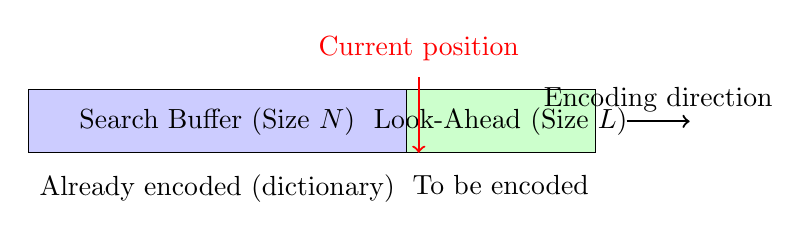
\begin{tikzpicture}[scale=0.8]
        % Search Buffer
        \draw[fill=blue!20] (0,0) rectangle (6,1);
        \node at (3,0.5) {Search Buffer (Size $N$)};
        
        % Look-Ahead Buffer
        \draw[fill=green!20] (6,0) rectangle (9,1);
        \node at (7.5,0.5) {Look-Ahead (Size $L$)};
        
        % Pointer
        \draw[->, thick, red] (6.2,1.2) -- (6.2,0);
        \node[above, red] at (6.2,1.3) {Current position};
        
        % Labels
        \node[below] at (3,-0.2) {Already encoded (dictionary)};
        \node[below] at (7.5,-0.2) {To be encoded};
        
        % Sliding direction
        \draw[->, thick] (9.5,0.5) -- (10.5,0.5);
        \node[above] at (10,0.5) {Encoding direction};
    \end{tikzpicture}
    \caption{LZ77 sliding window structure}
\end{figure}

\subsubsection{Encoding Tuples: (Offset, Length, Next Symbol)}

At each step, the encoder finds the longest match in the search buffer for the prefix of the look-ahead buffer. The match is encoded as:
\[
(\text{offset}, \text{length}, \text{next symbol})
\]
where:
\begin{itemize}
    \item \textbf{Offset}: Distance backward to the match (1-based indexing).
    \item \textbf{Length}: Number of matching symbols.
    \item \textbf{Next symbol}: The first symbol after the match (or EOF).
\end{itemize}

If no match is found, the encoder outputs $(0,0,c)$ where $c$ is the literal symbol from the look-ahead buffer.

\subsubsection{Step-by-Step Encoding Example}

Consider encoding the string \texttt{abracadabra} with a sufficiently large window:

\begin{center}
\begin{tabular}{cccl}
\toprule
Step & Search Buffer & Look-Ahead & Output \\
\midrule
1 & -- & \texttt{abracadabra} & $(0,0,\texttt{a})$ \\
2 & \texttt{a} & \texttt{bracadabra} & $(0,0,\texttt{b})$ \\
3 & \texttt{ab} & \texttt{racadabra} & $(0,0,\texttt{r})$ \\
4 & \texttt{abr} & \texttt{acadabra} & $(3,1,\texttt{c})$ \\
5 & \texttt{abrac} & \texttt{adabra} & $(5,1,\texttt{d})$ \\
6 & \texttt{abraca} & \texttt{abra} & $(7,4,\$)$ \\
\bottomrule
\end{tabular}
\end{center}

Where $\$$ denotes end-of-file. Notice how the second occurrence of "\texttt{abra}" (length 4) is encoded by referencing back to offset 7 (the first occurrence starting at position 1 in our 0-indexed string).

\subsubsection{Decoding Process: Simple Reconstruction}

Decoding is straightforward and proceeds sequentially:

\begin{algorithm}[H]
\caption{LZ77 Decoding}
\begin{algorithmic}[1]
\Procedure{Decode}{$stream$}
    \State Initialize output $\leftarrow$ empty string
    \For{each tuple $(o,l,c)$ in $stream$}
        \If{$o = 0$ and $l = 0$}
            \State Append $c$ to output
        \Else
            \State $start \leftarrow \text{length}(output) - o$
            \For{$i \leftarrow 0$ to $l-1$}
                \State Append output$[start + i]$ to output
            \EndFor
            \If{$c \neq \$ $}
                \State Append $c$ to output
            \EndIf
        \EndIf
    \EndFor
    \State \Return output
\EndProcedure
\end{algorithmic}
\end{algorithm}

\begin{examplebox}
\textbf{Decoding Example}:\\
Decoding the sequence from our example:
\begin{align*}
(0,0,\texttt{a}) &\rightarrow \texttt{a} \\
(0,0,\texttt{b}) &\rightarrow \texttt{ab} \\
(0,0,\texttt{r}) &\rightarrow \texttt{abr} \\
(3,1,\texttt{c}) &\rightarrow \texttt{abrac} \\
(5,1,\texttt{d}) &\rightarrow \texttt{abracad} \\
(7,4,\$) &\rightarrow \texttt{abracadabra}
\end{align*}
\end{examplebox}

\begin{importantbox}
\textbf{Why Decoding Works}: Every referenced symbol has already been reconstructed. The decoder maintains exactly the same output buffer that served as the encoder's search buffer.
\end{importantbox}

\subsubsection{Design Parameters: Window Size and Match Limits}

LZ77 has two key parameters:
\begin{itemize}
    \item \textbf{Search buffer size ($N$)}: Larger buffers find more matches but increase memory and search time.
    \item \textbf{Maximum match length ($L$)}: Limits how far ahead the encoder can look.
\end{itemize}

Practical implementations use efficient data structures (hash tables, suffix arrays) to find matches in $O(1)$ or $O(\log N)$ time rather than the naive $O(NL)$.

\subsection{LZSS: Improving Practical Efficiency}

Published in 1982 by James Storer and Thomas Szymanski, LZSS addresses a key inefficiency in LZ77.

\subsubsection{The Problem with LZ77's Encoding}

LZ77's $(o,l,c)$ format has two inefficiencies:
\begin{enumerate}
    \item \textbf{No-match penalty}: $(0,0,c)$ uses more bits than the literal $c$ alone.
    \item \textbf{Short-match penalty}: Encoding a match of length 2 might not save bits after accounting for tuple overhead.
\end{enumerate}

\subsubsection{Flag Bits: Literal vs. Match}

LZSS introduces a \textbf{flag bit} preceding each encoded element:
\begin{itemize}
    \item \textbf{Flag = 0}: Next item is a literal symbol (8 bits for ASCII).
    \item \textbf{Flag = 1}: Next item is a match pair (offset, length).
\end{itemize}

\begin{importantbox}
\textbf{Key Insight}: LZSS separates the \emph{parsing decision} ("literal or match?") from the \emph{data encoding} itself. This conceptual separation is crucial for understanding modern hybrid compressors.
\end{importantbox}

\begin{figure}[H]
    \centering
    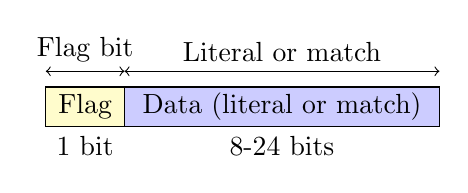
\begin{tikzpicture}
        % Flag bit
        \draw[fill=yellow!20] (0,0) rectangle (1,0.5);
        \node at (0.5,0.25) {Flag};
        
        % Data
        \draw[fill=blue!20] (1,0) rectangle (5,0.5);
        \node at (3,0.25) {Data (literal or match)};
        
        % Labels
        \node[below] at (0.5,0) {1 bit};
        \node[below] at (3,0) {8-24 bits};
        
        \draw[<->] (0,0.7) -- (1,0.7);
        \node[above] at (0.5,0.7) {Flag bit};
        
        \draw[<->] (1,0.7) -- (5,0.7);
        \node[above] at (3,0.7) {Literal or match};
    \end{tikzpicture}
    \caption{LZSS encoding format}
\end{figure}

\subsubsection{Match Threshold}

LZSS introduces a \textbf{match threshold}: only encode matches that are \emph{long enough} to actually save bits. Typically:

\[
\text{Encode match if: } l \times \text{bits\_per\_symbol} > \text{bits\_for\_flag} + \text{bits\_for\_offset} + \text{bits\_for\_length}
\]

For typical parameters (8-bit symbols, 12-bit offset, 4-bit length):
\[
\text{Match if: } l \times 8 > 1 + 12 + 4 = 17 \implies l \geq 3
\]

So LZSS would only encode matches of length 3 or more.

\subsubsection{LZSS Encoding Example}

Let's encode \texttt{abracadabra} with LZSS (match threshold = 3):

\begin{center}
\begin{tabular}{cccc}
\toprule
Step & Look-Ahead & Action & Output \\
\midrule
1 & \texttt{abracadabra} & No match $\geq 3$ & Flag=0, \texttt{a} \\
2 & \texttt{bracadabra} & No match $\geq 3$ & Flag=0, \texttt{b} \\
3 & \texttt{racadabra} & No match $\geq 3$ & Flag=0, \texttt{r} \\
4 & \texttt{acadabra} & Match "\texttt{a}" (length=1) & Flag=0, \texttt{a} \\
5 & \texttt{cadabra} & No match $\geq 3$ & Flag=0, \texttt{c} \\
6 & \texttt{adabra} & Match "\texttt{a}" (length=1) & Flag=0, \texttt{a} \\
7 & \texttt{dabra} & No match $\geq 3$ & Flag=0, \texttt{d} \\
8 & \texttt{abra} & Match "\texttt{abra}" (length=4) & Flag=1, (7,4) \\
\bottomrule
\end{tabular}
\end{center}

Output in binary (simplified):
\begin{itemize}
    \item Flag bits: 0 0 0 0 0 0 0 1
    \item Literals: a b r a c a d
    \item Match: offset=7, length=4
\end{itemize}

\subsubsection{Why LZSS Matters}

\begin{importantbox}
LZSS is the foundation for the \textbf{DEFLATE} algorithm used in ZIP files, gzip, PNG images, and HTTP compression. Its innovations---flag bits and match thresholds---make dictionary compression practical for real-world use.
\end{importantbox}

\subsection{LZ78: The Dictionary Growth Algorithm}

Published in 1978, LZ78 takes a different approach: it builds an explicit dictionary that grows as encoding proceeds.

\subsubsection{Building an Explicit Dictionary from Scratch}

Unlike LZ77's sliding window, LZ78 builds a dictionary of phrases:
\begin{itemize}
    \item Starts with empty dictionary (index 0 represents empty string).
    \item Each new phrase is added to the dictionary.
    \item Dictionary indices are assigned sequentially.
\end{itemize}

\subsubsection{Encoding Pairs: (Dictionary Index, New Symbol)}

LZ78 outputs pairs:
\[
(\text{index}, \text{symbol})
\]
where:
\begin{itemize}
    \item \textbf{Index}: Dictionary index of the longest matching prefix.
    \item \textbf{Symbol}: The next symbol after the match.
\end{itemize}

The new phrase (dictionary[index] + symbol) is added to the dictionary.

\begin{algorithm}[H]
\caption{LZ78 Encoding}
\begin{algorithmic}[1]
\Procedure{Encode}{$input$}
    \State Initialize dict $\leftarrow \{\epsilon\}$ (empty string at index 0)
    \State $current \leftarrow \epsilon$
    
    \For{each symbol $s$ in $input$}
        \If{$current + s$ is in dict}
            \State $current \leftarrow current + s$
        \Else
            \State $i \leftarrow$ index of $current$ in dict
            \State Output $(i, s)$
            \State Add $current + s$ to dict
            \State $current \leftarrow \epsilon$
        \EndIf
    \EndFor
    
    \If{$current \neq \epsilon$}
        \State Output $(index(current), \$)$
    \EndIf
\EndProcedure
\end{algorithmic}
\end{algorithm}

\subsubsection{Worked Example: From String to Codes}

Encoding \texttt{abracadabra}:

\begin{center}
\begin{tabular}{cccc}
\toprule
Step & Current Phrase & Output & New Dictionary Entry \\
\midrule
1 & \texttt{a} & $(0,\texttt{a})$ & 1: \texttt{a} \\
2 & \texttt{b} & $(0,\texttt{b})$ & 2: \texttt{b} \\
3 & \texttt{r} & $(0,\texttt{r})$ & 3: \texttt{r} \\
4 & \texttt{ac} & $(1,\texttt{c})$ & 4: \texttt{ac} \\
5 & \texttt{ad} & $(1,\texttt{d})$ & 5: \texttt{ad} \\
6 & \texttt{abr} & $(1,\texttt{b})$ & 6: \texttt{ab} \\
\bottomrule
\end{tabular}
\end{center}

The output sequence: $(0,a)$, $(0,b)$, $(0,r)$, $(1,c)$, $(1,d)$, $(1,b)$.

\subsubsection{Comparison with LZ77/LZSS}

\begin{importantbox}
\textbf{LZ78 vs LZ77/LZSS}:
\begin{itemize}
    \item \textbf{LZ77/LZSS}: Fast adaptation, limited memory (window), good for local repeats.
    \item \textbf{LZ78}: Slow start, unlimited growth, captures long-term repetitions.
    \item In practice, LZ77/LZSS variants dominate due to better memory behavior and faster adaptation.
\end{itemize}
\end{importantbox}

\subsection{Theoretical Properties: Why Lempel--Ziv Works}

\subsubsection{The Universality Principle}

Lempel--Ziv algorithms have a remarkable theoretical property:

\begin{definitionbox}
\textbf{Universal Compression}: An algorithm is universal if it can compress any stationary ergodic source to its entropy rate \emph{without prior knowledge} of the source statistics.
\end{definitionbox}

Both LZ77 and LZ78 are universal compressors.

\subsubsection{Asymptotic Optimality}

\begin{theorem}[Ziv \& Lempel, 1977-1978]
For any stationary ergodic source with entropy rate $H$, let $L_n$ be the length of the LZ77 or LZ78 encoding of $n$ source symbols. Then:
\[
\lim_{n \to \infty} \frac{\mathbb{E}[L_n]}{n} = H
\]
\end{theorem}

\begin{proof}[Intuition]
As $n$ grows large:
\begin{itemize}
    \item The algorithm sees enough repetitions to build an accurate implicit model.
    \item Common phrases get short codes (through references).
    \item Rare phrases get longer codes (literal transmission).
    \item The average code length approaches the self-information of phrases.
\end{itemize}
\end{proof}

\subsubsection{Practical Implications of Universality}

\begin{importantbox}
\textbf{Why Universality Matters}:
\begin{itemize}
    \item No need to estimate probabilities or build explicit models.
    \item Works on any data type (text, images, executables, DNA).
    \item Adapts automatically to source characteristics.
    \item Explains why LZ methods work so well in practice.
\end{itemize}
\end{importantbox}

\subsection{Bridging Paradigms: Dictionary vs. Entropy Coding}

\subsubsection{Complementary Approaches}

Dictionary coding and entropy coding address different aspects of compression:
\begin{itemize}
    \item \textbf{Dictionary coding}: Exploits \emph{structural redundancy} (repetitions).
    \item \textbf{Entropy coding}: Exploits \emph{statistical redundancy} (skewed symbol frequencies).
\end{itemize}

\subsubsection{The Hybrid Approach}

Modern compressors combine both approaches:

\begin{figure}[H]
    \centering
    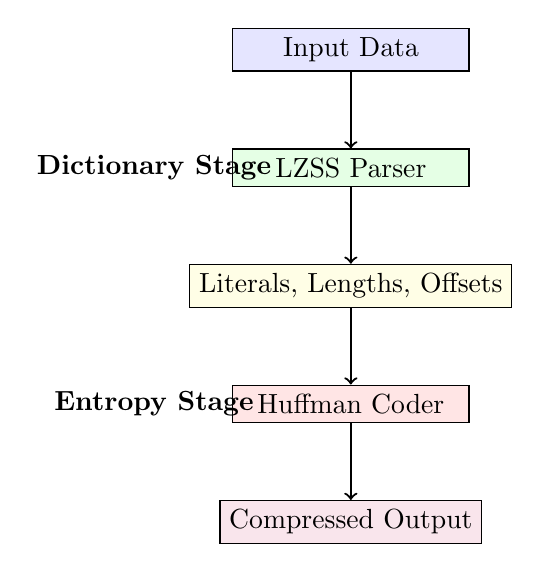
\begin{tikzpicture}[node distance=1.5cm]
        % Nodes
        \node (input) [rectangle, draw, fill=blue!10, minimum width=3cm] {Input Data};
        \node (lzss) [rectangle, draw, fill=green!10, minimum width=3cm, below of=input] {LZSS Parser};
        \node (stream) [rectangle, draw, fill=yellow!10, minimum width=3cm, below of=lzss] {Literals, Lengths, Offsets};
        \node (huffman) [rectangle, draw, fill=red!10, minimum width=3cm, below of=stream] {Huffman Coder};
        \node (output) [rectangle, draw, fill=purple!10, minimum width=3cm, below of=huffman] {Compressed Output};
        
        % Arrows
        \draw[->, thick] (input) -- (lzss);
        \draw[->, thick] (lzss) -- (stream);
        \draw[->, thick] (stream) -- (huffman);
        \draw[->, thick] (huffman) -- (output);
        
        % Labels
        \node[left of=lzss, xshift=-1cm] {\textbf{Dictionary Stage}};
        \node[left of=huffman, xshift=-1cm] {\textbf{Entropy Stage}};
    \end{tikzpicture}
    \caption{Hybrid compression pipeline (e.g., DEFLATE algorithm)}
\end{figure}

The DEFLATE algorithm (used in ZIP, PNG, gzip) works precisely this way:
\begin{enumerate}
    \item LZSS finds repeated strings, outputs literals and matches.
    \item Huffman coding compresses:
    \begin{itemize}
        \item Literal symbols (0-255)
        \item Match lengths (257-285)
        \item Match distance codes (0-29)
    \end{itemize}
\end{enumerate}

\subsection{Summary and Forward Look}

\subsubsection{Key Takeaways}

\begin{itemize}
    \item \textbf{Paradigm shift}: Dictionary coding exploits repetition rather than probabilities.
    \item \textbf{LZ77}: Sliding window approach, encodes matches as triples.
    \item \textbf{LZSS}: Practical improvement with flag bits and match thresholds.
    \item \textbf{LZ78}: Explicit dictionary growth, encodes pairs.
    \item \textbf{Universality}: LZ methods work on any stationary source without prior knowledge.
    \item \textbf{Modern practice}: Hybrid systems (LZSS + Huffman) dominate.
\end{itemize}

\subsubsection{The Road Ahead: DEFLATE and Beyond}

In our next lecture, we'll study the DEFLATE algorithm in detail:
\begin{itemize}
    \item How LZSS and Huffman coding are combined.
    \item The gzip/ZIP/PNG compression pipeline.
    \item Practical implementation considerations.
    \item Performance trade-offs and optimizations.
\end{itemize}

\begin{importantbox}
\textbf{Historical Context}: The Lempel--Ziv papers (1977, 1978) are among the most cited in information theory. Their algorithms underpin much of today's digital compression infrastructure. Understanding these foundations is essential for working with modern compression standards.
\end{importantbox}

% ================= END OF CHAPTER EXERCISES =================

\subsection*{End of Chapter Exercises}

\begin{exercisebox}
\textbf{Exercise 5.1 (LZ77 Encoding)}\\
Encode the string \texttt{TOBEORNOTTOBEORTOBEORNOT} using LZ77 with a search buffer of size 12. Show your work step by step with the search buffer, look-ahead buffer, and output tuples.
\end{exercisebox}

\begin{exercisebox}
\textbf{Exercise 5.2 (LZSS Efficiency Analysis)}\\
Compare LZ77 and LZSS for encoding a sequence with parameters: 8-bit symbols, 12-bit offsets, 4-bit lengths.
\begin{enumerate}[label=(\alph*)]
    \item How many bits does LZ77 use for a non-match?
    \item How many bits does LZSS use for a literal?
    \item What is the minimum match length that saves bits in LZSS?
    \item When would LZ77 be more efficient than LZSS?
\end{enumerate}
\end{exercisebox}

\begin{exercisebox}
\textbf{Exercise 5.3 (LZ78 Dictionary Growth)}\\
Encode the string \texttt{ABABABABA} using LZ78. Show the dictionary after each step and the complete output sequence. How many dictionary entries are created?
\end{exercisebox}

\begin{exercisebox}
\textbf{Exercise 5.4 (Algorithm Comparison)}\\
For each string below, predict which would perform better: LZ77/LZSS or LZ78? Explain why.
\begin{enumerate}[label=(\alph*)]
    \item \texttt{AAAAAAAAAAAAAAAAAAAA} (20 A's)
    \item \texttt{ABCDEFGHIJKLMNOPQRSTUVWXYZ}
    \item \texttt{ABABABABABABABABABAB}
    \item A file containing the same 1KB block repeated 100 times
\end{enumerate}
\end{exercisebox}

\begin{exercisebox}
\textbf{Exercise 5.5 (Decoding Challenge)}\\
Decode the following LZSS encoded sequence (match threshold = 3):
\begin{verbatim}
0 T
0 H
0 E
1 (3,5)
0 _
0 _
1 (5,4)
0 .
\end{verbatim}
Where: 
- Each line represents one encoded element
- Flag 0 indicates a literal character
- Flag 1 indicates a match (offset, length)
- \_ represents space character
- . represents period

What is the original string? Show your decoding step by step.
\end{exercisebox}

\begin{exercisebox}
\textbf{Exercise 5.6 (Window Size Analysis)}\\
Consider LZ77 with search buffer size $N$.
\begin{enumerate}[label=(\alph*)]
    \item How many bits are needed to encode an offset value?
    \item If we increase $N$ from 4096 to 65536, how many more bits are needed for offsets?
    \item What is the trade-off in choosing $N$?
    \item In practice, why might we choose $N = 32768$ over $N = 65536$ even if memory is available?
\end{enumerate}
\end{exercisebox}

\begin{exercisebox}
\textbf{Exercise 5.7 (Universal Compression Intuition)}\\
Explain in your own words why Lempel--Ziv algorithms are universal. Why don't they need to know source statistics in advance? How do they "learn" the source structure?
\end{exercisebox}

\begin{exercisebox}
\textbf{Exercise 5.8 (Hybrid Coding Design)}\\
Design a simple hybrid compressor that:
\begin{enumerate}[label=(\alph*)]
    \item Uses LZSS with match threshold 3
    \item Collects statistics on literals, lengths, and offsets
    \item Applies Huffman coding to each alphabet separately
\end{enumerate}
How would the decoder know which Huffman trees to use?
\end{exercisebox}

\begin{exercisebox}
\textbf{Exercise 5.9 (Search Efficiency)}\\
A naive LZ77 implementation searches for matches by comparing the look-ahead buffer against every position in the search buffer.
\begin{enumerate}[label=(\alph*)]
    \item What is the time complexity of this approach?
    \item Describe how a hash table can improve search efficiency.
    \item What information would you store in the hash table?
    \item How would you handle hash collisions?
\end{enumerate}
\end{exercisebox}

\begin{exercisebox}
\textbf{Exercise 5.10 (Theoretical Limits)}\\
Prove or provide intuition for:
\begin{enumerate}[label=(\alph*)]
    \item LZ77 cannot achieve compression ratio better than the entropy rate for i.i.d. sources.
    \item LZ78 may perform poorly on very short inputs.
    \item For sources with long-range dependencies, LZ methods can outperform block Huffman coding even with large blocks.
\end{enumerate}
\end{exercisebox}


\end{document}
